% defer/rcuusage.tex
% mainfile: ../perfbook.tex
% SPDX-License-Identifier: CC-BY-SA-3.0

\subsection{RCU Usage}
\label{sec:defer:RCU Usage}
\OriginallyPublished{Section}{sec:defer:RCU Usage}{RCU Usage}{Linux Weekly News}{PaulEMcKenney2008WhatIsRCUUsage}

This section answers the question ``What is RCU?'' from the viewpoint
of the uses to which RCU can be put.
Because RCU is most frequently used to replace some existing mechanism,
we look at it primarily in terms of its relationship to such mechanisms,
as listed in \cref{tab:defer:RCU Usage}
and as displayed in \cref{fig:defer:Relationships Between RCU Use Cases}.
Following the sections listed in this table,
\cref{sec:defer:RCU Usage Summary} provides a summary.

\begin{table}
\renewcommand*{\arraystretch}{1.2}
\centering
\small
\begin{tabular}{ll}
\toprule
Mechanism RCU Replaces & Page \\
\midrule
RCU for pre-BSD routing &
	\pageref{sec:defer:RCU for Pre-BSD Routing} \\
Wait for pre-existing things to finish &
	\pageref{sec:defer:Wait for Pre-Existing Things to Finish} \\
Phased state change &
	\pageref{sec:defer:Phased State Change} \\
Add-only list (publish/subscribe) &
	\pageref{sec:defer:Add-Only List} \\
Type-safe memory &
	\pageref{sec:defer:Type-Safe Memory} \\
Existence Guarantee &
	\pageref{sec:defer:Existence Guarantee} \\
Light-weight garbage collector &
	\pageref{sec:defer:Light-Weight Garbage Collector} \\
Delete-only list &
	\pageref{sec:defer:Delete-Only List} \\
Quasi reader-writer lock &
	\pageref{sec:defer:Quasi Reader-Writer Lock} \\
Quasi reference count &
	\pageref{sec:defer:Quasi Reference Count} \\
Quasi multi-version concurrency control (MVCC) &
	\pageref{sec:defer:Quasi Multi-Version Concurrency Control} \\
\bottomrule
\end{tabular}
\caption{RCU Usage}
\label{tab:defer:RCU Usage}
\end{table}

\subsubsection{RCU for Pre-BSD Routing}
\label{sec:defer:RCU for Pre-BSD Routing}

In contrast to the later sections, this section focuses on a very
specific use case for the purpose of comparison with other mechanisms.

\Cref{lst:defer:RCU Pre-BSD Routing Table Lookup,%
lst:defer:RCU Pre-BSD Routing Table Add/Delete}
show code for an RCU-protected Pre-BSD routing table
(\path{route_rcu.c}).
The former shows data structures and \co{route_lookup()},
and the latter shows \co{route_add()} and \co{route_del()}.

\begin{listing}
\input{CodeSamples/defer/route_rcu@lookup.fcv}
\caption{RCU Pre-BSD Routing Table Lookup}
\label{lst:defer:RCU Pre-BSD Routing Table Lookup}
\end{listing}

\begin{listing}
\input{CodeSamples/defer/route_rcu@add_del.fcv}
\caption{RCU Pre-BSD Routing Table Add/Delete}
\label{lst:defer:RCU Pre-BSD Routing Table Add/Delete}
\end{listing}

\begin{fcvref}[ln:defer:route_rcu:lookup]
In \cref{lst:defer:RCU Pre-BSD Routing Table Lookup},
\clnref{rh} adds the \co{->rh} field used by RCU reclamation,
\clnref{re_freed} adds the \co{->re_freed} use-after-free-check field,
\clnref{lock,unlock1,unlock2}
add RCU read-side protection,
and \clnref{chk_freed,abort} add the use-after-free check.
\end{fcvref}
\begin{fcvref}[ln:defer:route_rcu:add_del]
In \cref{lst:defer:RCU Pre-BSD Routing Table Add/Delete},
\clnref{add:lock,add:unlock,del:lock,%
del:unlock1,del:unlock2} add update-side locking,
\clnref{add:add_rcu,del:del_rcu} add RCU update-side protection,
\clnref{del:call_rcu} causes \co{route_cb()} to be invoked after
a grace period elapses,
and \clnrefrange{cb:b}{cb:e} define \co{route_cb()}.
This is minimal added code for a working concurrent implementation.
\end{fcvref}

\begin{figure}
\centering
\resizebox{2.5in}{!}{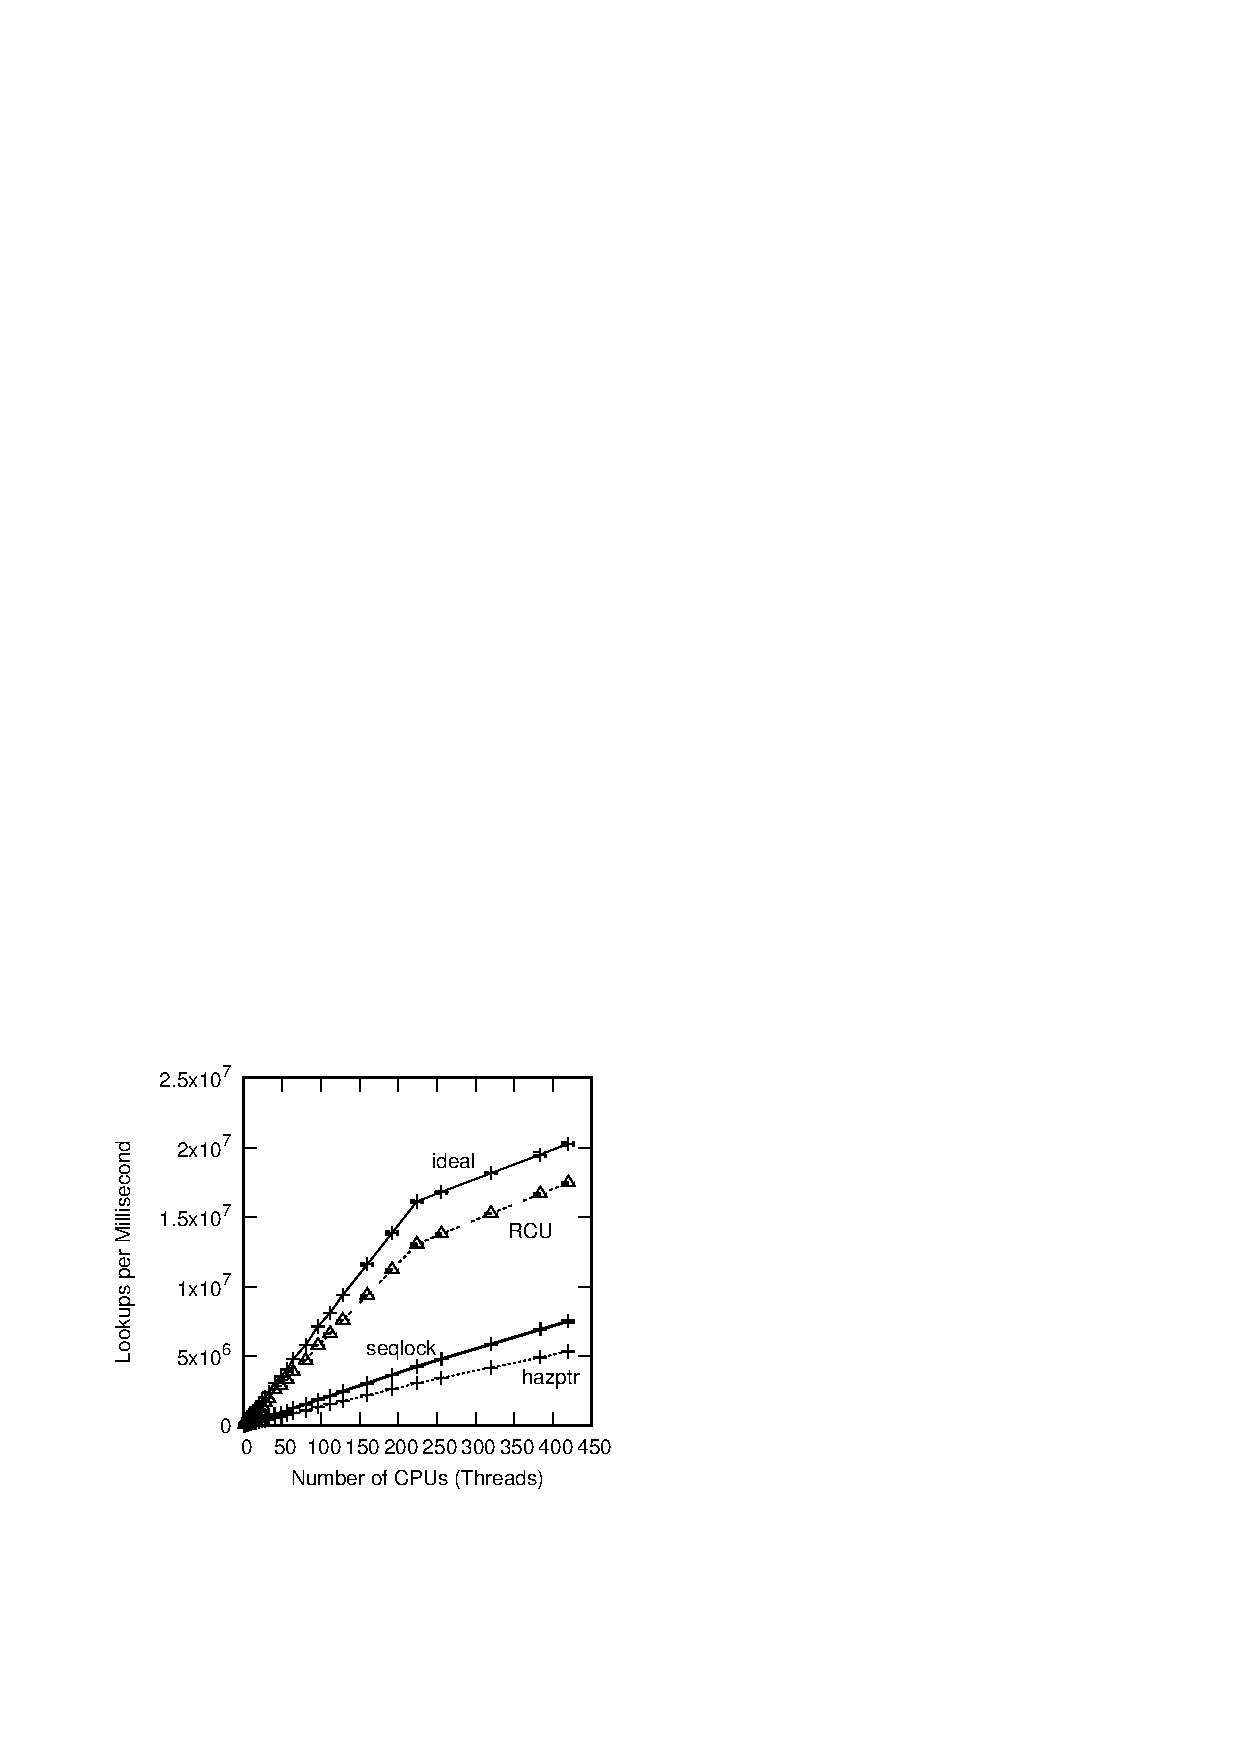
\includegraphics{CodeSamples/defer/data/hps.2019.12.17a/perf-rcu}}
\caption{Pre-BSD Routing Table Protected by RCU}
\label{fig:defer:Pre-BSD Routing Table Protected by RCU}
\end{figure}

\Cref{fig:defer:Pre-BSD Routing Table Protected by RCU}
shows the performance on the read-only workload.
RCU scales quite well, and offers nearly ideal performance.
However, this data was generated using the \co{RCU_SIGNAL}
flavor of userspace
RCU~\cite{MathieuDesnoyers2009URCU,PaulMcKenney2013LWNURCU},
for which \co{rcu_read_lock()} and \co{rcu_read_unlock()}
generate a small amount of code.
What happens for the \IXacr{qsbr} flavor of RCU, which generates no code at all
for \co{rcu_read_lock()} and \co{rcu_read_unlock()}?
(See \cref{sec:defer:Introduction to RCU},
and especially
\cref{fig:defer:QSBR: Waiting for Pre-Existing Readers},
for a discussion of RCU QSBR\@.)

The answer to this is shown in
\cref{fig:defer:Pre-BSD Routing Table Protected by RCU QSBR},
which shows that RCU QSBR's performance and scalability actually exceeds
that of the ideal synchronization-free workload.

\QuickQuizSeries{%
\QuickQuizB{
	Wait, what???
	How can RCU QSBR possibly be better than ideal?
	Just what rubbish definition of ideal would fail to be the best
	of all possible results???
}\QuickQuizAnswerB{
	This is an excellent question, and the answer is that modern
	CPUs and compilers are extremely complex.
	But before getting into that, it is well worth noting that
	RCU QSBR's performance advantage appears only in the
	one-hardware-thread-per-core regime.
	Once the system is fully loaded, RCU QSBR's performance drops
	back to ideal.

	The RCU variant of the \co{route_lookup()} search loop actually
	has one more x86 instruction than does the sequential version,
	namely the \co{lea} in the sequence
	\co{cmp}, \co{je}, \co{mov}, \co{cmp}, \co{lea}, and \co{jne}.
	This extra instruction is due to the \co{rcu_head} structure
	at the beginning of the RCU variant's \co{route_entry} structure,
	so that, unlike the sequential variant, the RCU variant's
	\co{->re_next.next} pointer has a non-zero offset.
	Back in the 1980s, this additional \co{lea} instruction might
	have reliably resulted in the RCU variant being slower, but we
	are now in the 21\textsuperscript{st} century, and the 1980s
	are long gone.

	But those of you who read
	\cref{sec:cpu:Pipelined CPUs}
	carefully already knew all of this!

	These counter-intuitive results of course means that any
	performance result on modern microprocessors must be subject to
	some skepticism.
	In theory, it really does not make sense to obtain performance
	results that are better than ideal, but it really can happen
	on modern microprocessors.
	Such results can be thought of as similar to the celebrated
	super-linear speedups (see
	\cref{sec:SMPdesign:Beyond Partitioning}
	for one such example), that is, of interest but also of limited
	practical importance.
	Nevertheless, one of the strengths of RCU is that its read-side
	overhead is so low that tiny effects such as this one are visible
	in real performance measurements.

\begin{figure}
\centering
% Run with initial rcu_head structure in route_entry moved down.
\resizebox{2.5in}{!}{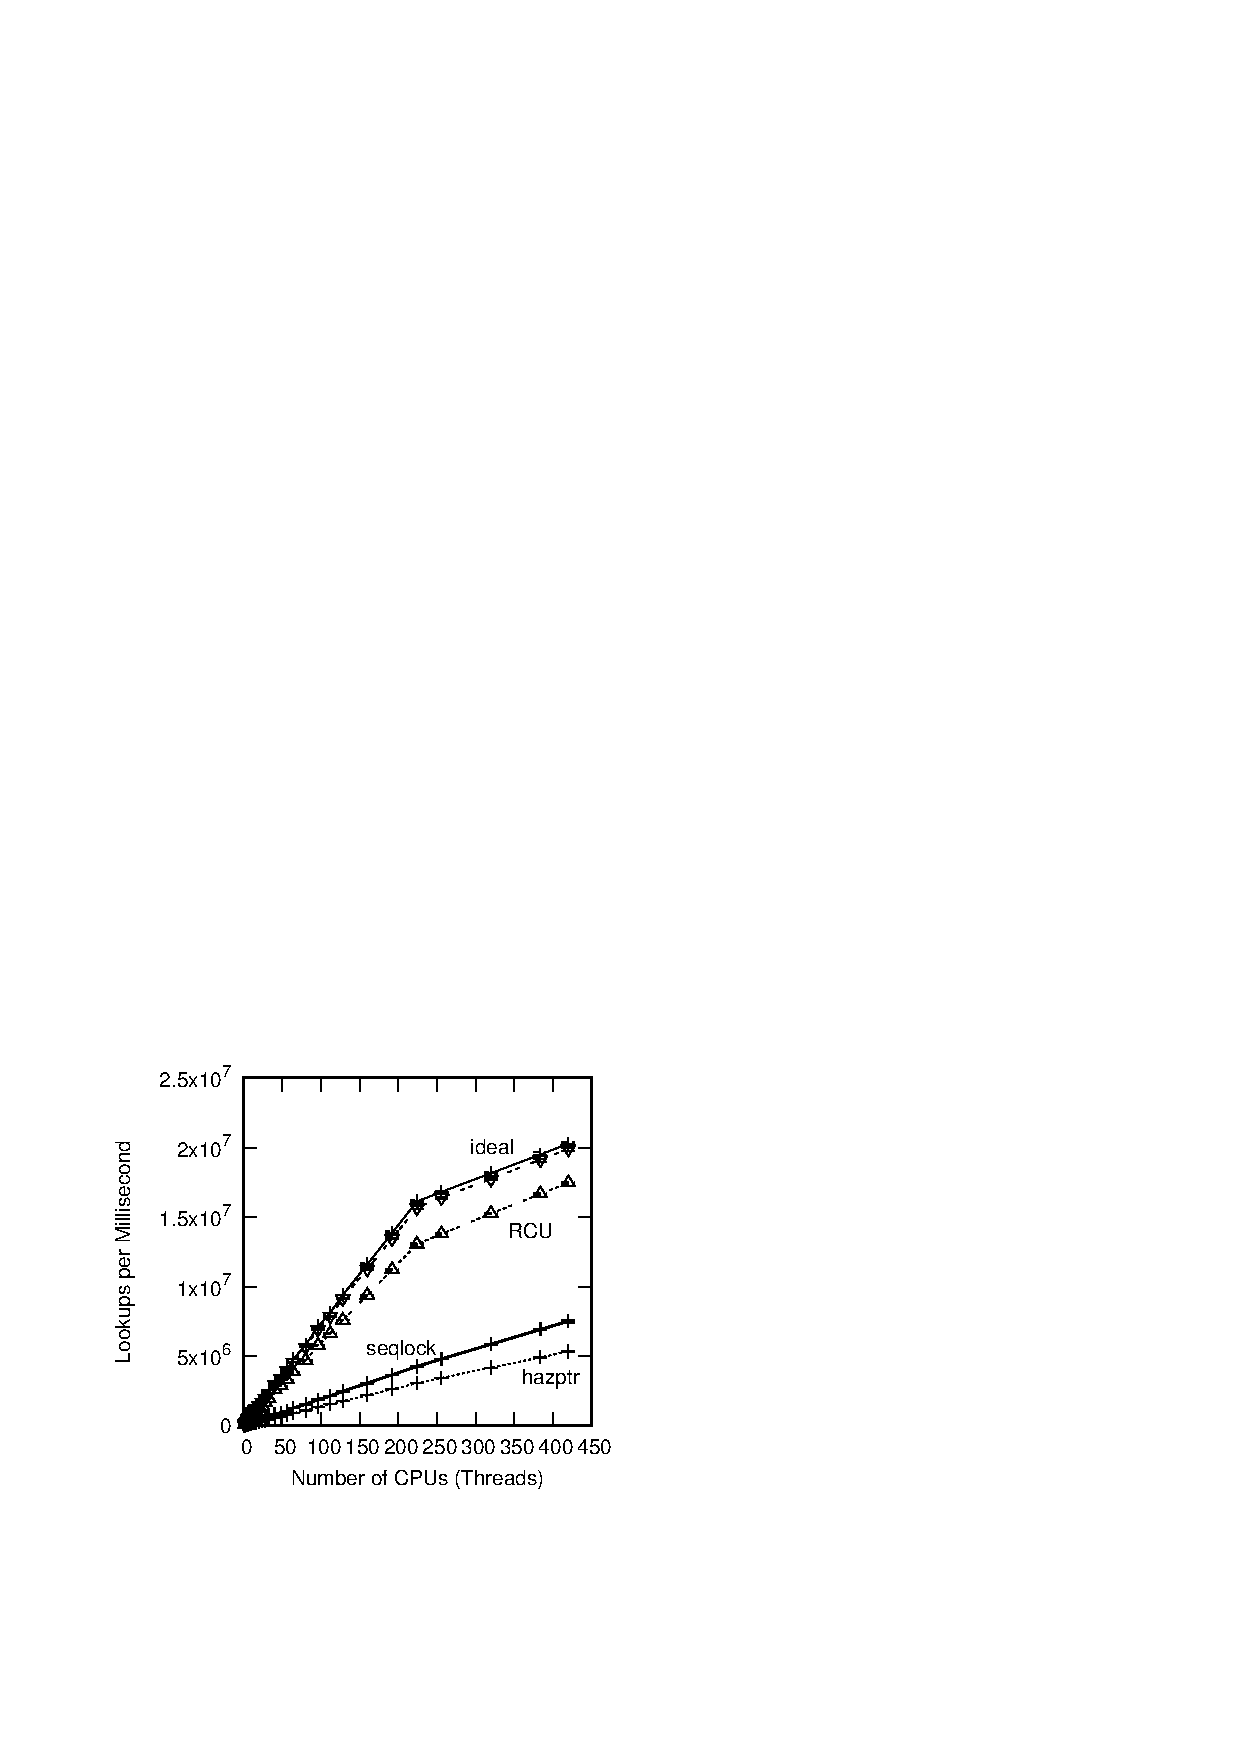
\includegraphics{CodeSamples/defer/data/hps.2019.12.17a/perf-rcu-qsbr}}
\caption{Pre-BSD Routing Table Protected by RCU QSBR With Non-Initial \tco{rcu_head}}
\label{fig:defer:Pre-BSD Routing Table Protected by RCU QSBR With Non-Initial rcu-head}
\end{figure}

	This raises the question as to what would happen if the
	\co{rcu_head} structure were to be moved so that RCU's
	\co{->re_next.next} pointer also had zero offset, just the
	same as the sequential variant.
	And the answer, as can be seen in
	\cref{fig:defer:Pre-BSD Routing Table Protected by RCU QSBR With Non-Initial rcu-head},
	is that this causes RCU QSBR's performance to decrease to where
	it is still very nearly ideal, but no longer super-ideal.
}\QuickQuizEndB
%
\QuickQuizE{
	Given RCU QSBR's read-side performance, why bother with any
	other flavor of userspace RCU?
}\QuickQuizAnswerE{
	Because RCU QSBR places constraints on the overall application
	that might not be tolerable,
	for example, requiring that each and every thread in the
	application regularly pass through a quiescent state.
	Among other things, this means that RCU QSBR is not helpful
	to library writers, who might be better served by other
	flavors of userspace RCU~\cite{PaulMcKenney2013LWNURCU}.
}\QuickQuizEndE
}

\begin{figure}
\centering
% Run with initial rcu_head structure at beginning of route_entry structure.
% This need to run twice is the reason for the oddball directory.
% @@@ Make this generate both files with a single run?
\resizebox{2.5in}{!}{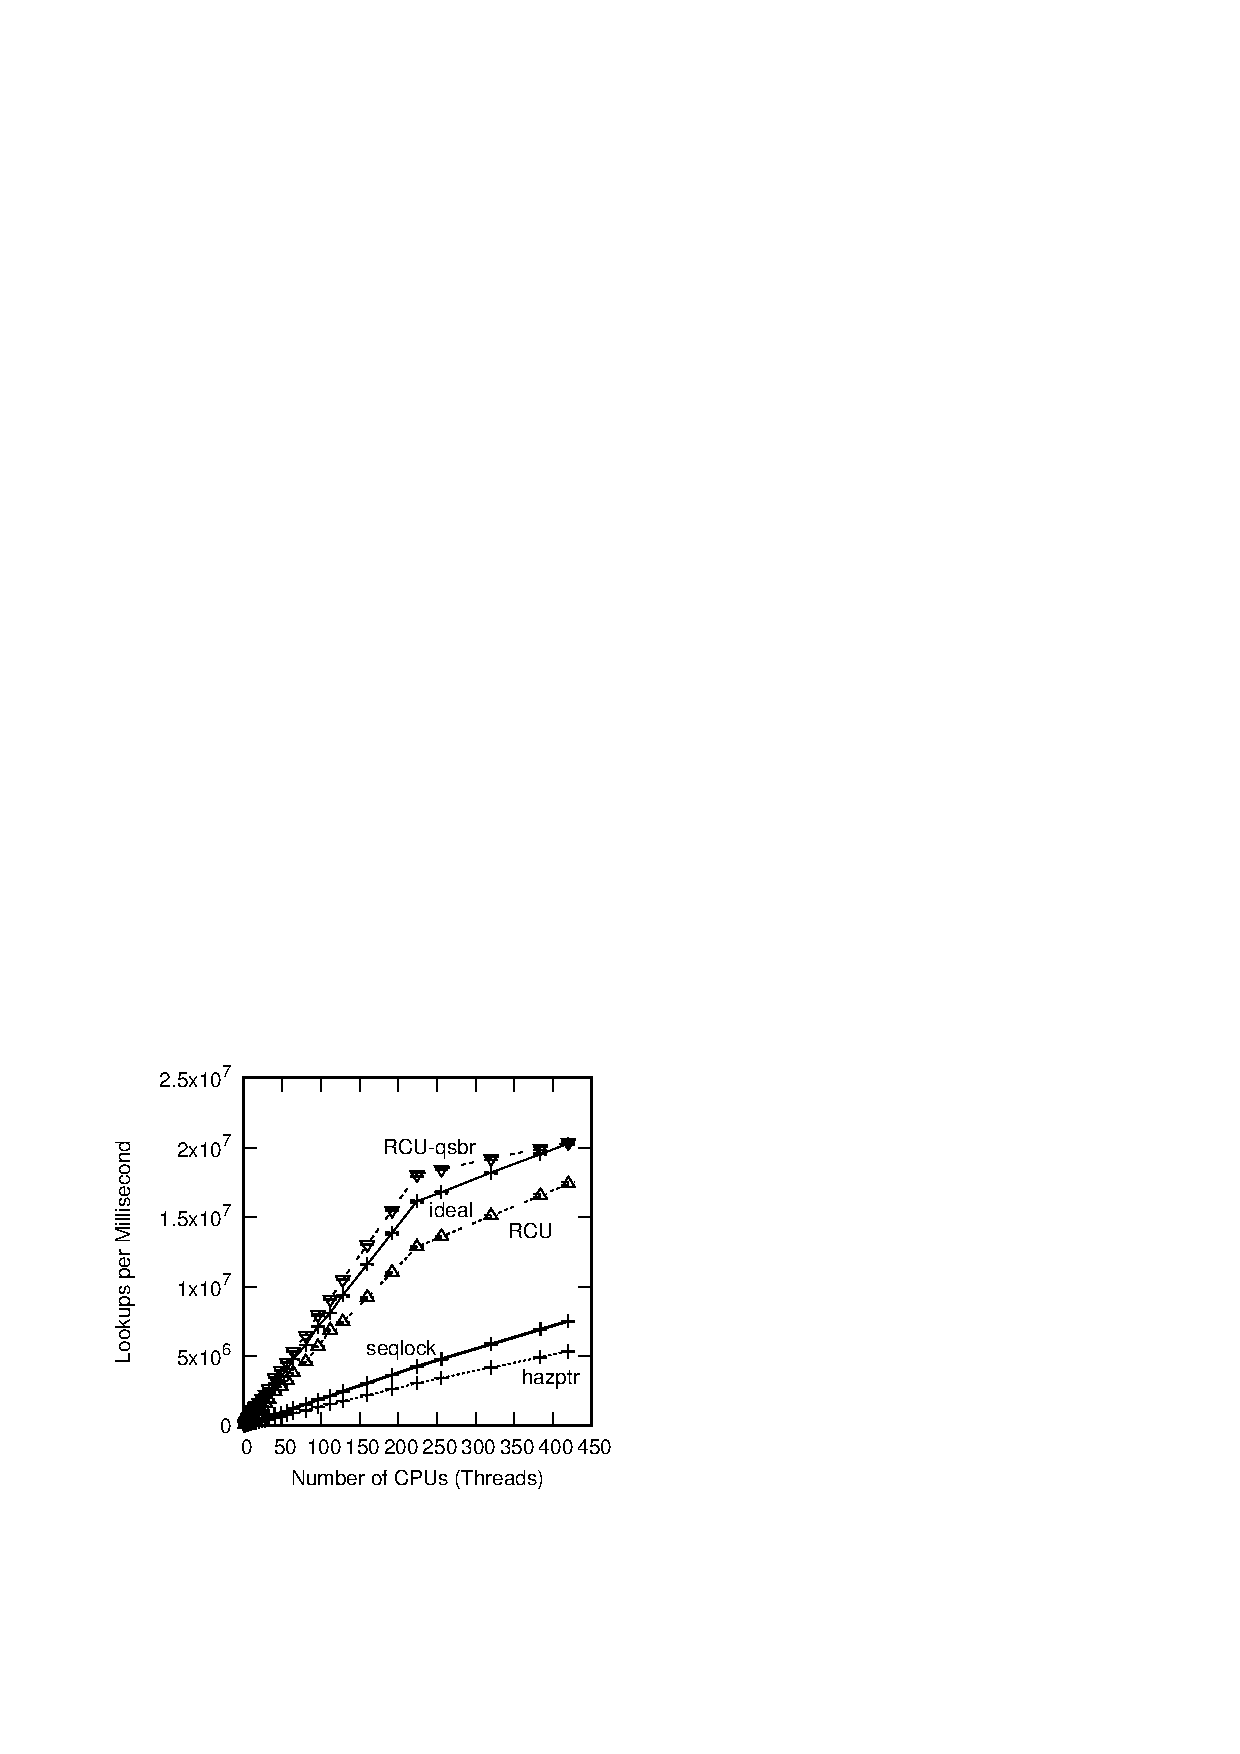
\includegraphics{CodeSamples/defer/data/hps.2019.12.02a/perf-rcu-qsbr}}
\caption{Pre-BSD Routing Table Protected by RCU QSBR}
\label{fig:defer:Pre-BSD Routing Table Protected by RCU QSBR}
\end{figure}

\begin{figure*}
\centering
\IfTwoColumn{
  \resizebox{5.5in}{!}{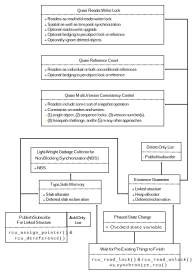
\includegraphics{defer/RCUusecases}}
}{
  \resizebox{.96\textwidth}{!}{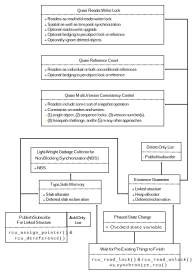
\includegraphics{defer/RCUusecases}}
  % eb builds require .96
}
\caption{Relationships Between RCU Use Cases}
\label{fig:defer:Relationships Between RCU Use Cases}
\end{figure*}

Although Pre-BSD routing is an excellent RCU use case, it is worthwhile
looking at the relationships betweeen the wider spectrum of use cases
shown in
\cref{fig:defer:Relationships Between RCU Use Cases}.
This task is taken up by the following sections.

While reading these sections, please ask yourself which of these
use cases best describes Pre-BSD routing.

\subsubsection{Wait for Pre-Existing Things to Finish}
\label{sec:defer:Wait for Pre-Existing Things to Finish}

As noted in \cref{sec:defer:RCU Fundamentals}
an important component
of RCU is a way of waiting for RCU readers to finish.
One of
RCU's great strength is that it allows you to wait for each of
thousands of different things to finish without having to explicitly
track each and every one of them, and without incurring
the performance degradation, scalability limitations, complex deadlock
scenarios, and memory-leak hazards that are inherent in schemes that
use explicit tracking.

In this section, we will show how \co{synchronize_sched()}'s
read-side counterparts (which include anything that disables preemption,
along with hardware operations and
primitives that disable interrupts) permit you to interaction with
non-maskable interrupt
(NMI) handlers, which is quite difficult using locking.
This approach has been called ``Pure RCU''~\cite{PaulEdwardMcKenneyPhD},
and it is used in a few places in the Linux kernel.

The basic form of such ``Pure RCU'' designs is as follows:

\begin{enumerate}
\item	Make a change, for example, to the way that the OS reacts to an NMI\@.
\item	Wait for all pre-existing read-side critical sections to
	completely finish (for example, by using the
	\co{synchronize_sched()} primitive).\footnote{
		In Linux kernel v5.1 and later, \co{synchronize_sched()} has
		been subsumed into \co{synchronize_rcu()}.}
	The key observation here is that subsequent RCU read-side critical
	sections are guaranteed to see whatever change was made.
\item	Clean up, for example, return status indicating that the
	change was successfully made.
\end{enumerate}

The remainder of this section presents example code adapted from
the Linux kernel.
In this example, the \co{nmi_stop()} function in the now-defunct
oprofile facility uses \co{synchronize_sched()} to ensure that all
in-flight NMI notifications have completed before freeing the associated
resources.
A simplified version of this code is shown in
\cref{lst:defer:Using RCU to Wait for NMIs to Finish}.

\begin{listing}
\begin{fcvlabel}[ln:defer:Using RCU to Wait for NMIs to Finish]
\begin{VerbatimL}[commandchars=\\\@\$]
struct profile_buffer {				\lnlbl@struct:b$
	long size;
	atomic_t entry[0];
};						\lnlbl@struct:e$
static struct profile_buffer *buf = NULL;	\lnlbl@struct:buf$

void nmi_profile(unsigned long pcvalue)		\lnlbl@nmi_profile:b$
{
	struct profile_buffer *p = rcu_dereference(buf);\lnlbl@nmi_profile:rcu_deref$

	if (p == NULL)				\lnlbl@nmi_profile:if_NULL$
		return;				\lnlbl@nmi_profile:ret:a$
	if (pcvalue >= p->size)			\lnlbl@nmi_profile:if_oor$
		return;				\lnlbl@nmi_profile:ret:b$
	atomic_inc(&p->entry[pcvalue]);		\lnlbl@nmi_profile:inc$
}						\lnlbl@nmi_profile:e$

void nmi_stop(void)				\lnlbl@nmi_stop:b$
{
	struct profile_buffer *p = buf;		\lnlbl@nmi_stop:fetch$

	if (p == NULL)				\lnlbl@nmi_stop:if_NULL$
		return;				\lnlbl@nmi_stop:ret$
	rcu_assign_pointer(buf, NULL);		\lnlbl@nmi_stop:NULL$
	synchronize_sched();			\lnlbl@nmi_stop:sync_sched$
	kfree(p);				\lnlbl@nmi_stop:kfree$
}						\lnlbl@nmi_stop:e$
\end{VerbatimL}
\end{fcvlabel}
\caption{Using RCU to Wait for NMIs to Finish}
\label{lst:defer:Using RCU to Wait for NMIs to Finish}
\end{listing}

\begin{fcvref}[ln:defer:Using RCU to Wait for NMIs to Finish:struct]
\Clnrefrange{b}{e} define a \co{profile_buffer} structure, containing a
size and an indefinite array of entries.
\Clnref{buf} defines a pointer to a profile buffer, which is
presumably initialized elsewhere to point to a dynamically allocated
region of memory.
\end{fcvref}

\begin{fcvref}[ln:defer:Using RCU to Wait for NMIs to Finish:nmi_profile]
\Clnrefrange{b}{e} define the \co{nmi_profile()} function,
which is called from within an NMI handler.
As such, it cannot be preempted, nor can it be interrupted by a normal
interrupt handler, however, it is still subject to delays due to cache misses,
ECC errors, and cycle stealing by other hardware threads within the same
core.
\Clnref{rcu_deref} gets a local pointer to the profile buffer using the
\co{rcu_dereference()} primitive to ensure memory ordering on
DEC Alpha, and
\clnref{if_NULL,ret:a} exit from this function if there is no
profile buffer currently allocated, while \clnref{if_oor,ret:b}
exit from this function if the \co{pcvalue} argument
is out of range.
Otherwise, \clnref{inc} increments the profile-buffer entry indexed
by the \co{pcvalue} argument.
Note that storing the size with the buffer guarantees that the
range check matches the buffer, even if a large buffer is suddenly
replaced by a smaller one.
\end{fcvref}

\begin{fcvref}[ln:defer:Using RCU to Wait for NMIs to Finish:nmi_stop]
\Clnrefrange{b}{e} define the \co{nmi_stop()} function,
where the caller is responsible for mutual exclusion (for example,
holding the correct lock).
\Clnref{fetch} fetches a pointer to the profile buffer, and
\clnref{if_NULL,ret} exit the function if there is no buffer.
Otherwise, \clnref{NULL} \co{NULL}s out the profile-buffer pointer
(using the \co{rcu_assign_pointer()} primitive to maintain
memory ordering on weakly ordered machines),
and \clnref{sync_sched} waits for an RCU Sched grace period to elapse,
in particular, waiting for all non-preemptible regions of code,
including NMI handlers, to complete.
Once execution continues at \clnref{kfree}, we are guaranteed that
any instance of \co{nmi_profile()} that obtained a
pointer to the old buffer has returned.
It is therefore safe to free the buffer, in this case using the
\co{kfree()} primitive.
\end{fcvref}

\QuickQuiz{
	Suppose that the \co{nmi_profile()} function was preemptible.
	What would need to change to make this example work correctly?
}\QuickQuizAnswer{
	One approach would be to use
	\co{rcu_read_lock()} and \co{rcu_read_unlock()}
	in \co{nmi_profile()}, and to replace the
	\co{synchronize_sched()} with \co{synchronize_rcu()},
	perhaps as shown in
	\cref{lst:defer:Using RCU to Wait for Mythical Preemptible NMIs to Finish}.
%
\begin{listing}
\begin{VerbatimL}
struct profile_buffer {
	long size;
	atomic_t entry[0];
};
static struct profile_buffer *buf = NULL;

void nmi_profile(unsigned long pcvalue)
{
	struct profile_buffer *p;

	rcu_read_lock();
	p = rcu_dereference(buf);
	if (p == NULL) {
		rcu_read_unlock();
		return;
	}
	if (pcvalue >= p->size) {
		rcu_read_unlock();
		return;
	}
	atomic_inc(&p->entry[pcvalue]);
	rcu_read_unlock();
}

void nmi_stop(void)
{
	struct profile_buffer *p = buf;

	if (p == NULL)
		return;
	rcu_assign_pointer(buf, NULL);
	synchronize_rcu();
	kfree(p);
}
\end{VerbatimL}
\caption{Using RCU to Wait for Mythical Preemptible NMIs to Finish}
\label{lst:defer:Using RCU to Wait for Mythical Preemptible NMIs to Finish}
\end{listing}

	But why on earth would an NMI handler be preemptible???
}\QuickQuizEnd

In short, RCU makes it easy to dynamically switch among profile
buffers (you just \emph{try} doing this efficiently with atomic
operations, or at all with locking!).
This is a rare use of RCU in its pure form.
RCU is normally used at higher levels of abstraction, as
will be shown in the following sections.

\subsubsection{Phased State Change}
\label{sec:defer:Phased State Change}

\Cref{fig:defer:Phased State Change for Maintenance Operation}
shows a timeline for an example phased state change to efficiently
handle maintenance operations.
If there is no maintenance operation in progress, common-case operations
must proceed quickly, for example, without acquiring a reader-writer lock.
However, if there is a maintenance operation in progress, the common-case
operations must be undertaken carefully, taking into account added
complexities due to their running concurrently with that maintenance
operation.
This means that common-case operations will incur higher overhead during
maintenance operations, which is one reason that maintenance operations
are normally scheduled to take place during times of low load.

\begin{figure}
\centering
\resizebox{\twocolumnwidth}{!}{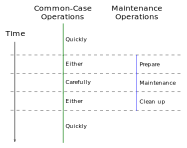
\includegraphics{defer/RCUphasedstatechange}}
\caption{Phased State Change for Maintenance Operation}
\label{fig:defer:Phased State Change for Maintenance Operation}
\end{figure}

In the figure, these apparently conflicting requirements are resolved by
having a prepare phase prior to the maintenance operation and a cleanup
phase after it, during which the common-case operations can proceed
either quickly or carefully.

\begin{listing}
\begin{fcvlabel}[ln:defer:Phased State Change for Maintenance Operations]
\begin{VerbatimL}[commandchars=\\\@\$]
bool be_careful;

void cco(void)
{
	rcu_read_lock();			\lnlbl@rrl$
	if (READ_ONCE(be_careful))		\lnlbl@if$
		cco_carefully();		\lnlbl@careful$
	else
		cco_quickly();			\lnlbl@quick$
	rcu_read_unlock();			\lnlbl@rul$
}

void maint(void)
{
	WRITE_ONCE(be_careful, true);		\lnlbl@tocareful$
	synchronize_rcu();			\lnlbl@sr1$
	do_maint();				\lnlbl@maint$
	synchronize_rcu();			\lnlbl@sr2$
	WRITE_ONCE(be_careful, false);		\lnlbl@toquick$
}
\end{VerbatimL}
\end{fcvlabel}
\caption{Phased State Change for Maintenance Operations}
\label{lst:defer:Phased State Change for Maintenance Operations}
\end{listing}

\begin{fcvref}[ln:defer:Phased State Change for Maintenance Operations]
Example pseudo-code for this phased state change is shown in
\cref{lst:defer:Phased State Change for Maintenance Operations}.
The common-case operations are carried out by \co{cco()} within an RCU
read-side critical section extending from \clnref{rrl} to \clnref{rul}.
Here, \clnref{if} checks a global \co{be_careful} flag, invoking
\co{cco_carefully()} or \co{cco_quickly()}, as indicated.
\end{fcvref}

\begin{fcvref}[ln:defer:Phased State Change for Maintenance Operations]
This allows the \co{maint()} function to set the \co{be_careful} flag
on \clnref{tocareful} and wait for an RCU grace period on \clnref{sr1}.
When control reaches \clnref{maint}, all \co{cco()} functions that saw a
\co{false} value of \co{be_careful} (and thus which might invoke
the \co{cco_quickly()} function) will have completed their operations,
so that all currently executing \co{cco()} functions will be invoking
\co{cco_carefully()}.
This means that it is safe for the \co{do_maint()} function to be
invoked.
\Clnref{sr2} then waits for all \co{cco()} functions that might have
run concurrently with \co{do_maint()} to complete, and finally
\clnref{toquick} sets the \co{be_careful} flag back to \co{false}.
\end{fcvref}

\QuickQuizSeries{%
\QuickQuizB{
	What is the point of the second call to \co{synchronize_rcu()}
	in function
	\co{maint()} in \cref{lst:defer:Phased State Change for Maintenance Operations}?
	Isn't it OK for any \co{cco()} invocations in the clean-up
	phase to invoke either \co{cco_carefully()} or \co{cco_quickly()}?
}\QuickQuizAnswerB{
	The problem is that there is no ordering between the \co{cco()}
	function's load from \co{be_careful} and any memory loads
	executed by the \co{cco_quickly()} function.
	Because there is no ordering, without that second call to
	\co{syncrhonize_rcu()}, memory ordering could cause loads
	in \co{cco_quickly()} to overlap with stores by \co{do_maint()}.

	Another alternative would be to compensate for the removal of
	that second call to \co{synchronize_rcu()} by changing the
	\co{READ_ONCE()} to \co{smp_load_acquire()} and the
	\co{WRITE_ONCE()} to \co{smp_store_release()}, thus restoring
	the needed ordering.
}\QuickQuizEndB

\QuickQuizE{
	How can you be sure that the code shown in
	\co{maint()} in \cref{lst:defer:Phased State Change for Maintenance Operations}
	really works?\@
}\QuickQuizAnswerE{
	By one popular school of thought, you cannot.

	But in this case, those willing to jump ahead to
	\cref{chp:Formal Verification}
	and
	\cref{chp:Advanced Synchronization: Memory Ordering}
	might find a couple of LKMM litmus tests to be interesting
	(\path{C-RCU-phased-state-change-1.litmus} and
	\path{C-RCU-phased-state-change-2.litmus}).
	These tests could be argued to demonstrate that this code
	and a variant of it really do work.
}\QuickQuizEndE
}% End of \QuickQuizSeries

Phased state change allows frequent operations to use light-weight
checks, without the need for expensive lock acquisitions or atomic
read-modify-write operations, and is used in the Linux kernel in the
guise of \co{rcu_sync}~\cite{OlegNesterov2013rcusync} to implement a
variant of reader-writer semaphores with lightweight readers.
Phased state change adds only a checked state variable
to the wait-to-finish use case
(\cref{sec:defer:Wait for Pre-Existing Things to Finish}),
thus also residing at a rather low level of abstraction.

\subsubsection{Add-Only List}
\label{sec:defer:Add-Only List}

Add-only data structures, exemplified by the add-only list, can be used
for a surprisingly common set of use cases, perhaps most commonly the
logging of changes.
Add-only data structures are a pure use of RCU's underlying
publish/subscribe mechanism.

An add-only variant of a pre-BSD routing table can be derived from
\cref{lst:defer:RCU Pre-BSD Routing Table Lookup,lst:defer:RCU Pre-BSD Routing Table Add/Delete}.
Because there is no deletion, the \co{route_del()} and \co{route_cb()}
functions may be dispensed with, along with the \co{->rh}
and \co{->re_freed} fields of the \co{route_entry} structure, the
\co{rcu_read_lock()}, the \co{rcu_read_unlock()} invocations in the
\co{route_lookup()} function, and all uses of the \co{->re_freed} field
in all remaining functions.

Of course, if there are many concurrent invocations of the \co{route_add()}
function, there will be heavy contention on \co{routelock}, and if lockless
techniques are used, heavy memory contention on \co{routelist}.
The usual way to avoid this contention is to use a concurrency-friendly
data structure such as a hash table (see \cref{chp:Data Structures}).
Alternatively, per-CPU data structures might be periodically merged
into a single global data structure.

On the other hand, if there is never any deletion, extended time periods
featuring many concurrent invocations of \co{route_add()} will eventually
consume all available memory.
Therefore, most RCU-protected data structures also implement deletion.

\subsubsection{Type-Safe Memory}
\label{sec:defer:Type-Safe Memory}

A number of lockless algorithms do not require that a given data
element keep the same identity through a given RCU read-side critical
section referencing it---but only if that data element retains the
same type.
In other words, these lockless algorithms can tolerate a given data
element being freed and reallocated as the same type of structure
while they are referencing it, but must prohibit a change in type.
This guarantee, called ``\IX{type-safe memory}'' in
academic literature~\cite{Cheriton96a},
is weaker than the \IXpl{existence guarantee} discussed
in \cref{sec:defer:Existence Guarantee},
and is therefore quite a bit harder to work with.
Type-safe memory algorithms in the Linux kernel make use of slab caches,
specially marking these caches with \co{SLAB_TYPESAFE_BY_RCU}
so that RCU is used when returning a freed-up
slab to system memory.
This use of RCU guarantees that any in-use element of
such a slab will remain in that slab, thus retaining its type,
for the duration of any pre-existing RCU read-side critical sections.

\QuickQuiz{
	But what if there is an arbitrarily long series of RCU
	read-side critical sections in multiple threads, so that at
	any point in time there is at least one thread in the system
	executing in an RCU read-side critical section?
	Wouldn't that prevent any data from a \co{SLAB_TYPESAFE_BY_RCU}
	slab ever being returned to the system, possibly resulting
	in OOM events?
}\QuickQuizAnswer{
	There could certainly be an arbitrarily long period of time
	during which at least one thread is always in an RCU read-side
	critical section.
	However, the key words in the description in
	\cref{sec:defer:Type-Safe Memory}
	are ``in-use'' and ``pre-existing''.
	Keep in mind that a given RCU read-side critical section is
	conceptually only permitted to gain references to data elements
	that were visible to readers during that critical section.
	Furthermore, remember that a slab cannot be returned to the
	system until all of its data elements have been freed, in fact,
	the RCU grace period cannot start until after they have all been
	freed.

	Therefore, the slab cache need only wait for those RCU read-side
	critical sections that started before the freeing of the last element
	of the slab.
	This in turn means that any RCU grace period that begins after
	the freeing of the last element will do---the slab may be returned
	to the system after that grace period ends.
}\QuickQuizEnd

It is important to note that \co{SLAB_TYPESAFE_BY_RCU} will
\emph{in no way}
prevent \co{kmem_cache_alloc()} from immediately reallocating
memory that was just now freed via \co{kmem_cache_free()}!
In fact, the \co{SLAB_TYPESAFE_BY_RCU}-protected data structure
just returned by \co{rcu_dereference()} might be freed and reallocated
an arbitrarily large number of times, even when under the protection
of \co{rcu_read_lock()}.
Instead, \co{SLAB_TYPESAFE_BY_RCU} operates by preventing
\co{kmem_cache_free()}
from returning a completely freed-up slab of data structures
to the system until after an RCU grace period elapses.
In short, although a given RCU read-side critical section might see a
given \co{SLAB_TYPESAFE_BY_RCU} data element being freed and reallocated
arbitrarily often, the element's type is guaranteed not to change until
that critical section has completed.

These algorithms therefore typically use a validation step that checks
to make sure that the newly referenced data structure really is the one
that was requested~\cite[Section~2.5]{LaninShasha1986TSM}.
These validation checks require that portions of the data structure
remain untouched by the free-reallocate process.
Such validation checks are usually very hard to get right, and can
hide subtle and difficult bugs.

Therefore, although type-safety-based lockless algorithms can be extremely
helpful in a very few difficult situations, you should instead use existence
guarantees where possible.
Simpler is after all almost always better!
On the other hand, type-safety-based lockless algorithms can
provide improved cache locality, and thus improved performance.
This improved cache locality is provided by the fact that such
algorithms can immediately reallocate a newly freed block of memory.
In contrast, algorithms based on existence guarantees must wait for
all pre-existing readers before reallocating memory, by which time
that memory may have been ejected from CPU caches.

As can be seen in \cref{fig:defer:Relationships Between RCU Use Cases},
RCU's type-safe-memory use case combines both the wait-to-finish
and publish-subscribe components, but in the Linux kernel also includes
the slab allocator's deferred reclamation specified by the
\co{SLAB_TYPESAFE_BY_RCU} flag.

\subsubsection{Existence Guarantee}
\label{sec:defer:Existence Guarantee}

Gamsa et al.~\cite{Gamsa99}
discuss \IXpl{existence guarantee} and describe how a mechanism
resembling RCU can be used to provide these existence guarantees
(see Section~5 on page~7 of the PDF), and
\cref{sec:locking:Lock-Based Existence Guarantees}
discusses how to guarantee existence via locking, along with the
ensuing disadvantages of doing so.
The effect is that if any RCU-protected data element is accessed
within an RCU read-side critical section, that data element is
guaranteed to remain in existence for the duration of that RCU
read-side critical section.

\begin{listing}
\begin{fcvlabel}[ln:defer:Existence Guarantees Enable Per-Element Locking]
\begin{VerbatimL}[commandchars=\\\@\$]
int delete(int key)
{
	struct element *p;
	int b;

	b = hashfunction(key);			\lnlbl@hash$
	rcu_read_lock();			\lnlbl@rdlock$
	p = rcu_dereference(hashtable[b]);
	if (p == NULL || p->key != key) {	\lnlbl@chkkey$
		rcu_read_unlock();		\lnlbl@rdunlock1$
		return 0;			\lnlbl@ret_0:a$
	}
	spin_lock(&p->lock);			\lnlbl@acq$
	if (hashtable[b] == p && p->key == key) {\lnlbl@chkkey2$
		rcu_read_unlock();		\lnlbl@rdunlock2$
		rcu_assign_pointer(hashtable[b], NULL);\lnlbl@remove$
		spin_unlock(&p->lock);		\lnlbl@rel1$
		synchronize_rcu();		\lnlbl@sync_rcu$
		kfree(p);			\lnlbl@kfree$
		return 1;			\lnlbl@ret_1$
	}
	spin_unlock(&p->lock);			\lnlbl@rel2$
	rcu_read_unlock();			\lnlbl@rdunlock3$
	return 0;				\lnlbl@ret_0:b$
}
\end{VerbatimL}
\end{fcvlabel}
\caption{Existence Guarantees Enable Per-Element Locking}
\label{lst:defer:Existence Guarantees Enable Per-Element Locking}
\end{listing}

\begin{fcvref}[ln:defer:Existence Guarantees Enable Per-Element Locking]
\Cref{lst:defer:Existence Guarantees Enable Per-Element Locking}
demonstrates how RCU-based existence guarantees can enable
per-element locking via a function that deletes an element from
a hash table.
\Clnref{hash} computes a hash function, and \clnref{rdlock} enters an RCU
read-side critical section.
If \clnref{chkkey} finds that the corresponding bucket of the hash table is
empty or that the element present is not the one we wish to delete,
then \clnref{rdunlock1} exits the RCU read-side critical section and
\clnref{ret_0:a}
indicates failure.
\end{fcvref}

\QuickQuiz{
	What if the element we need to delete is not the first element
	of the list on
	\clnrefr{ln:defer:Existence Guarantees Enable Per-Element Locking:chkkey} of
	\cref{lst:defer:Existence Guarantees Enable Per-Element Locking}?
}\QuickQuizAnswer{
	As with the (bug-ridden)
	\cref{lst:locking:Per-Element Locking Without Existence Guarantees (Buggy!)},
	this is a very simple hash table with no chaining, so the only
	element in a given bucket is the first element.
	The reader is again invited to adapt this example to a hash table with
	full chaining.
	Less energetic readers might wish to refer to
	\cref{chp:Data Structures}.
}\QuickQuizEnd

\begin{fcvref}[ln:defer:Existence Guarantees Enable Per-Element Locking]
Otherwise, \clnref{acq} acquires the update-side spinlock, and
\clnref{chkkey2} then checks that the element is still the one that we want.
If so, \clnref{rdunlock2} leaves the RCU read-side critical section,
\clnref{remove} removes it from the table, \clnref{rel1} releases
the lock, \clnref{sync_rcu} waits for all pre-existing RCU read-side critical
sections to complete, \clnref{kfree} frees the newly removed element,
and \clnref{ret_1} indicates success.
If the element is no longer the one we want, \clnref{rel2} releases
the lock, \clnref{rdunlock3} leaves the RCU read-side critical section,
and \clnref{ret_0:b} indicates failure to delete the specified key.
\end{fcvref}

\QuickQuizSeries{%
\QuickQuizB{
	\begin{fcvref}[ln:defer:Existence Guarantees Enable Per-Element Locking]
	Why is it OK to exit the RCU read-side critical section on
	\clnref{rdunlock2} of
	\cref{lst:defer:Existence Guarantees Enable Per-Element Locking}
	before releasing the lock on \clnref{rel1}?
	\end{fcvref}
}\QuickQuizAnswerB{
	\begin{fcvref}[ln:defer:Existence Guarantees Enable Per-Element Locking]
	First, please note that the second check on \clnref{chkkey2} is
	necessary because some other
	CPU might have removed this element while we were waiting
	to acquire the lock.
	However, the fact that we were in an RCU read-side critical section
	while acquiring the lock guarantees that this element could not
	possibly have been re-allocated and re-inserted into this
	hash table.
	Furthermore, once we acquire the lock, the lock itself guarantees
	the element's existence, so we no longer need to be in an
	RCU read-side critical section.

	The question as to whether it is necessary to re-check the
	element's key is left as an exercise to the reader.
	% A re-check is necessary if the key can mutate or if it is
	% necessary to reject deleted entries (in cases where deletion
	% is recorded by mutating the key.
	\end{fcvref}
}\QuickQuizEndB
%
\QuickQuizM{
	\begin{fcvref}[ln:defer:Existence Guarantees Enable Per-Element Locking]
	Why not exit the RCU read-side critical section on
	\clnref{rdunlock3} of
	\cref{lst:defer:Existence Guarantees Enable Per-Element Locking}
	before releasing the lock on \clnref{rel2}?
	\end{fcvref}
}\QuickQuizAnswerM{
	Suppose we reverse the order of these two lines.
	Then this code is vulnerable to the following sequence of
	events:
	\begin{enumerate}
	\begin{fcvref}[ln:defer:Existence Guarantees Enable Per-Element Locking]
	\item	CPU~0 invokes \co{delete()}, and finds the element
		to be deleted, executing through \clnref{rdunlock2}.
		It has not yet actually deleted the element, but
		is about to do so.
	\item	CPU~1 concurrently invokes \co{delete()}, attempting
		to delete this same element.
		However, CPU~0 still holds the lock, so CPU~1 waits
		for it at \clnref{acq}.
	\item	CPU~0 executes \clnref{remove,rel1},
		and blocks at \clnref{sync_rcu} waiting for CPU~1
		to exit its RCU read-side critical section.
	\item	CPU~1 now acquires the lock, but the test on \clnref{chkkey2}
		fails because CPU~0 has already removed the element.
		CPU~1 now executes \clnref{rel2}
		(which we switched with \clnref{rdunlock3}
		for the purposes of this Quick Quiz)
		and exits its RCU read-side critical section.
	\item	CPU~0 can now return from \co{synchronize_rcu()},
		and thus executes \clnref{kfree}, sending the element to
		the freelist.
	\item	CPU~1 now attempts to release a lock for an element
		that has been freed, and, worse yet, possibly
		reallocated as some other type of data structure.
		This is a fatal memory-corruption error.
	\end{fcvref}
	\end{enumerate}
}\QuickQuizEndM
%
\QuickQuizE{
	The RCU-based algorithm shown in
	\cref{lst:defer:Existence Guarantees Enable Per-Element Locking}
	locks very similar to that in
	\cref{lst:locking:Per-Element Locking With Lock-Based Existence Guarantees},
	so why should the RCU-based approach be any better?
}\QuickQuizAnswerE{
	\Cref{lst:defer:Existence Guarantees Enable Per-Element Locking}
	replaces the per-element \co{spin_lock()} and \co{spin_unlock()}
	shown in
	\cref{lst:locking:Per-Element Locking With Lock-Based Existence Guarantees}
	with a much cheaper \co{rcu_read_lock()} and \co{rcu_read_unlock()},
	thus greatly improving both performance and scalability.
	For more detail, please see
	\cref{sec:datastruct:RCU-Protected Hash Table Performance}.
}\QuickQuizEndE
}

Alert readers will recognize this as only a slight variation on
the original wait-to-finish theme
(\cref{sec:defer:Wait for Pre-Existing Things to Finish}),
adding publish/subscribe, linked structures, a heap allocator
(typically), and deferred reclamation, as shown in
\cref{fig:defer:Relationships Between RCU Use Cases}.
They might also note the deadlock-immunity advantages over the lock-based
existence guarantees discussed in
\cref{sec:locking:Lock-Based Existence Guarantees}.

\subsubsection{Light-Weight Garbage Collector}
\label{sec:defer:Light-Weight Garbage Collector}

A not-uncommon exclamation made by people first learning about
RCU is ``RCU is sort of like a garbage collector!''
This exclamation has a large grain of truth, but it can also be
misleading.

Perhaps the best way to think of the relationship between RCU
and automatic garbage collectors (GCs) is that RCU resembles
a GC in that the \emph{timing} of collection is automatically
determined, but that RCU differs from a GC in that:
\begin{enumerate*}[(1)]
\item The programmer must manually indicate when a given data
structure is eligible to be collected and
\item The programmer must manually mark the RCU read-side critical
sections where references might be held.
\end{enumerate*}

Despite these differences, the resemblance does go quite deep.
In fact, the first RCU-like mechanism I am aware of used a
reference-count-based garbage collector to handle the grace
periods~\cite{Kung80}, and the connection between RCU and
garbage collection has been noted more
recently~\cite{HarshalSheth2016goRCU}.

The light-weight garbage collector use case is very similar to
the existence-guarantee use case, adding only the desired non-blocking
algorithm to the mix.
This light-weight garbage collector use case can also be used in
conjunction with the existence guarantees described in the next section.

\subsubsection{Delete-Only List}
\label{sec:defer:Delete-Only List}

The delete-only list is the less-popular counterpart to the add-only list
covered in \cref{sec:defer:Add-Only List}, and can be thought of as the
existence-guarantee use case, but without the publish/subscribe component,
as shown in \cref{fig:defer:Relationships Between RCU Use Cases}.
A delete-only list can be used when the universe of possible members of
the list is known at initialization, and where members can be removed.
For example, elements of the list might represent hardware elements of
the system that are subject to failure, but cannot be repaired or
replaced without a reboot.

An delete-only variant of a pre-BSD routing table can be derived from
\cref{lst:defer:RCU Pre-BSD Routing Table Lookup,lst:defer:RCU Pre-BSD Routing Table Add/Delete}.
Because there is no addition, the \co{route_add()} function may be
dispensed with, or, alternatively, its use might be restricted to
initialization time.
In theory, the \co{route_lookup()} function can use a non-RCU iterator,
though in the Linux kernel this will result in complaints from debug code.
In addition, the incremental cost of an RCU iterator is usually
negligible.

As a result, delete-only situations typically use algorithms and data
structures that are designed for addition as well as deletion.

\subsubsection{Quasi Reader-Writer Lock}
\label{sec:defer:Quasi Reader-Writer Lock}

Perhaps the most common use of RCU within the Linux kernel is as
a replacement for reader-writer locking in read-intensive situations.
Nevertheless, this use of RCU was not immediately apparent to me
at the outset.
In fact, I chose to implement a lightweight reader-writer
lock~\cite{WilsonCHsieh92a}\footnote{
	Similar to \co{brlock} in the 2.4 Linux kernel and to
	\co{lglock} in more recent Linux kernels.}
before implementing a general-purpose RCU implementation
back in the early 1990s.
Each and every one of the uses I envisioned for the lightweight reader-writer
lock was instead implemented using RCU\@.
In fact, it was more than
three years before the lightweight reader-writer lock saw its first use.
Boy, did I feel foolish!

The key similarity between RCU and reader-writer locking is that
both have read-side critical sections that can execute concurrently.
In fact, in some cases, it is possible to mechanically substitute RCU API
members for the corresponding reader-writer lock API members.
But first, why bother?

Advantages of RCU include performance,
deadlock immunity, and realtime latency.
There are, of course, limitations to RCU, including the fact that
readers and updaters run concurrently, that low-priority RCU readers
can block high-priority threads waiting for a grace period to elapse,
and that grace-period latencies can extend for many milliseconds.
These advantages and limitations are discussed in the following paragraphs.

\paragraph{Performance}

\begin{figure}
\centering
\resizebox{2.5in}{!}{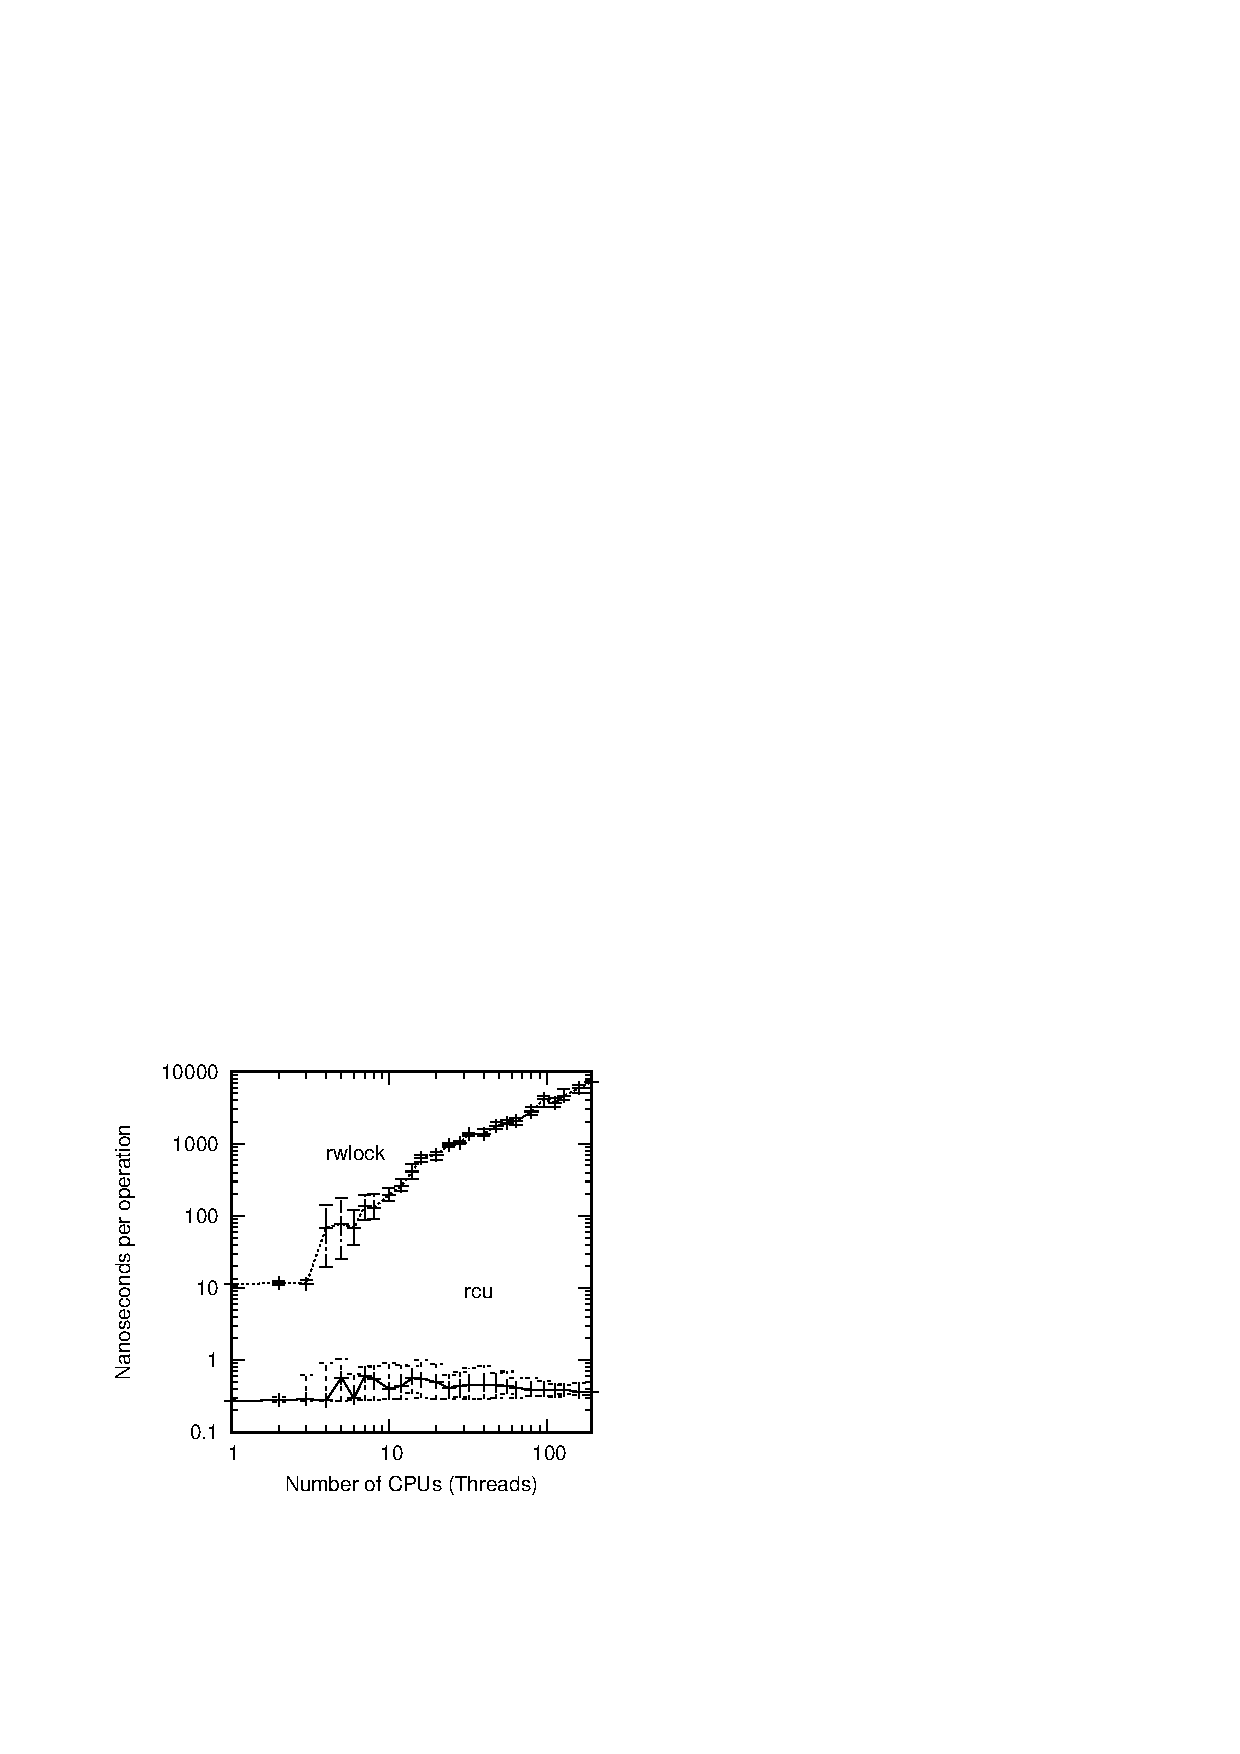
\includegraphics{CodeSamples/defer/data/rcuscale.hps.2020.05.28a/rwlockRCUperf}}
\caption{Performance Advantage of RCU Over Reader-Writer Locking}
\label{fig:defer:Performance Advantage of RCU Over Reader-Writer Locking}
\end{figure}

The read-side performance advantages of Linux-kernel RCU over
reader-writer locking are shown in
\cref{fig:defer:Performance Advantage of RCU Over Reader-Writer Locking},
which was generated on a 448-CPU 2.10\,GHz Intel x86 system.

\QuickQuizSeries{%
\QuickQuizB{
	WTF\@?
	How the heck do you expect me to believe that RCU can have less
	than a 300-picosecond overhead when the clock period at 2.10\,GHz
	is almost 500\,picoseconds?
}\QuickQuizAnswerB{
	First, consider that the inner loop used to
	take this measurement is as follows:

\begin{VerbatimN}
	for (i = nloops; i >= 0; i--) {
		rcu_read_lock();
		rcu_read_unlock();
	}
\end{VerbatimN}

	Next, consider the effective definitions of \co{rcu_read_lock()}
	and \co{rcu_read_unlock()}:

\begin{VerbatimN}
#define rcu_read_lock()   barrier()
#define rcu_read_unlock() barrier()
\end{VerbatimN}

	These definitions constrain compiler code-movement optimizations
	involving memory references, but emit no instructions in and
	of themselves.
	However, if the loop variable is maintained in a register,
	the accesses to \co{i} will not count as memory references.
	Furthermore, the compiler can do loop unrolling,
	allowing the resulting code to ``execute'' multiple passes
	through the loop body simply by incrementing \co{i} by
	some value larger than the value 1.

	So the ``measurement'' of 267 picoseconds is simply the fixed
	overhead of the timing measurements divided by the number of
	passes through the inner loop containing the calls
	to \co{rcu_read_lock()} and \co{rcu_read_unlock()}, plus
	the code to manipulate \co{i} divided by the loop-unrolling
	factor.
	And therefore, this measurement really is in error, in fact,
	it exaggerates the overhead by an arbitrary number of orders
	of magnitude.
	After all, in terms of machine instructions emitted, the actual
	overheads of \co{rcu_read_lock()} and of \co{rcu_read_unlock()}
	are each precisely zero.

	It is not just every day that a timing measurement of 267
	picoseconds turns out to be an overestimate!
}\QuickQuizEndB

\QuickQuizM{
	Didn't an earlier edition of this book show RCU read-side
	overhead way down in the sub-picosecond range?
	What happened???
}\QuickQuizAnswerM{
	Excellent memory!!!
	The overhead in some early releases was in fact roughly
	100~femtoseconds.

	What happened was that RCU usage spread more broadly through the
	Linux kernel, including into code that takes page faults.
	Back at that time, \co{rcu_read_lock()} and \co{rcu_read_unlock()}
	were complete no-ops in \co{CONFIG_PREEMPT=n} kernels.
	Unfortunately, that situation allowed the compiler to reorder
	page-faulting memory accesses into RCU read-side critical
	sections.
	Of course, page faults can block, which destroys those critical
	sections.

	Nor was this a theoretical problem:
	A failure actually manifested in 2019.
	\ppl{Herbert}{Xu} tracked down this failure down and
	\ppl{Linus}{Torvalds}
	therefore queued a commit to upgrade \co{rcu_read_lock()} and
	\co{rcu_read_unlock()} to unconditionally include a call to
	\co{barrier()}~\cite{LinusTorvalds2019:RCUreader.barrier}.
	And although \co{barrier()} emits no code, it does constrain
	compiler optimizations.
	And so the price of widespread RCU usage is slightly higher
	\co{rcu_read_lock()} and \co{rcu_read_unlock()} overhead.
	As such, Linux-kernel RCU has proven to be a victim of its
	own success.

	Of course, it is also the case that the older results were obtained
	on a different system than were those shown in
	\cref{fig:defer:Performance Advantage of RCU Over Reader-Writer Locking}.
	So which change had the most effect, Linus's commit or the change in
	the system?
	This question is left as an exercise to the reader.
}\QuickQuizEndM

\QuickQuizE{
	Why is there such large variation for the \co{RCU} trace in
	\cref{fig:defer:Performance Advantage of RCU Over Reader-Writer Locking}?
}\QuickQuizAnswerE{
	Keep in mind that this is a log-log plot, so those large-seeming
	\co{RCU} variances in reality span only a few hundred picoseconds.
	And that is such a short time that anything could cause it.
	However, given that the variance decreases with both small and
	large numbers of CPUs, one hypothesis is that the variation is
	due to migrations from one CPU to another.

	Yes, these measurements were taken with interrupts disabled, but
	they were also taken within a guest OS, so that preemption was
	still possible at the hypervisor level.
	In addition, the system featured hyperthreading and a single
	hardware thread running this RCU workload is able to consume
	more than half of the core's resources.
	Therefore, the overall throughput varies depending on how many
	of a given guest OS's CPUs share cores.
	Attempting to reduce these variations by running the guest OSes
	at real-time priority (as suggested by Joel Fernandes) is left
	as an exercise for the reader.
}\QuickQuizEndE
}                 % End of \QuickQuizSeries

Note that reader-writer locking is more than an order of magnitude slower
than RCU on a single CPU, and is more than \emph{four} orders of magnitude
slower on 192~CPUs.
In contrast, RCU scales quite well.
In both cases, the error bars cover the full range of the measurements
from 30~runs, with the line being the median.

\begin{figure}
\centering
\resizebox{2.5in}{!}{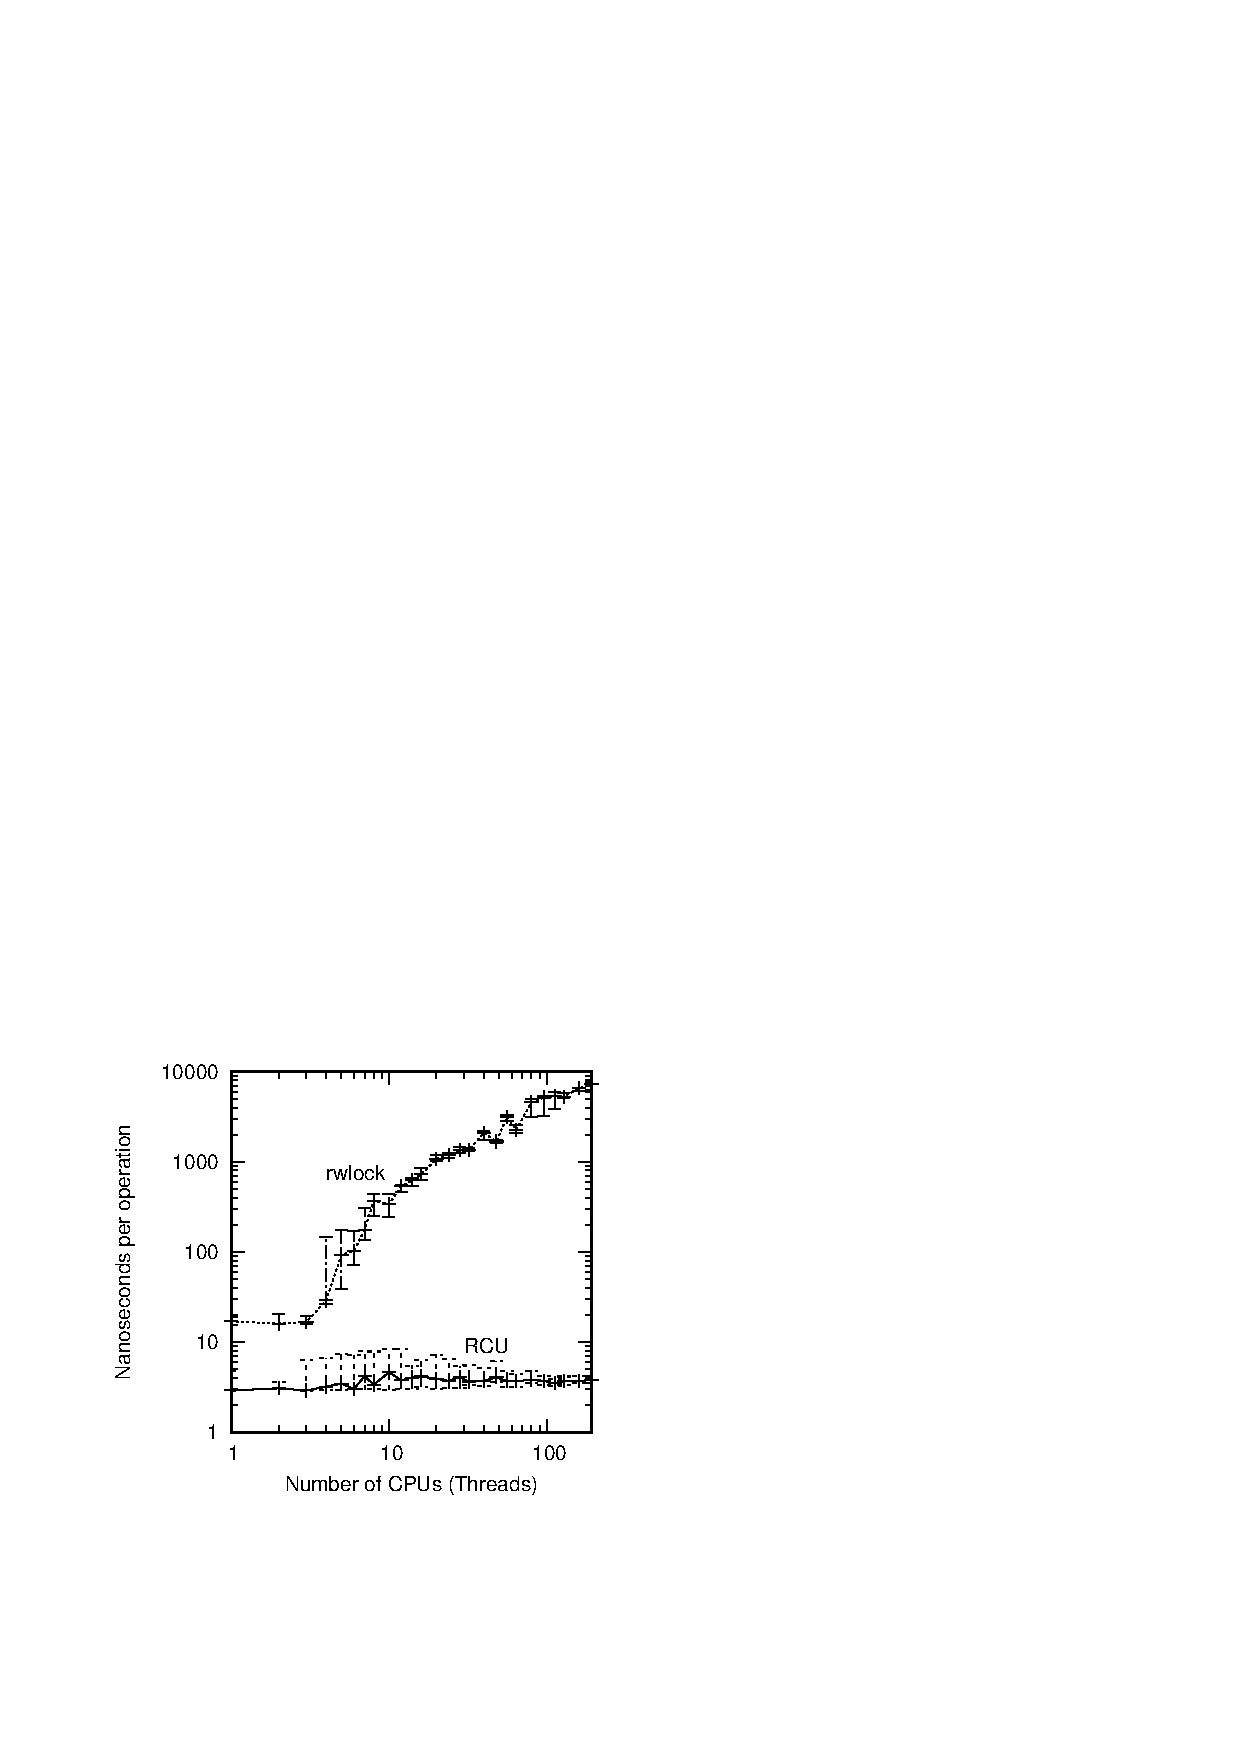
\includegraphics{CodeSamples/defer/data/rcuscale.hps.2020.05.28a/rwlockRCUperfPREEMPT}}
\caption{Performance Advantage of Preemptible RCU Over Reader-Writer Locking}
\label{fig:defer:Performance Advantage of Preemptible RCU Over Reader-Writer Locking}
\end{figure}

A more moderate view may be obtained from a \co{CONFIG_PREEMPT} kernel,
though RCU still beats reader-writer locking by between a factor of seven
on a single CPU and by three orders of magnitude on 192~CPUs, as shown in
\cref{fig:defer:Performance Advantage of Preemptible RCU Over Reader-Writer Locking},
which was generated on the same 448-CPU 2.10\,GHz x86 system.
Note the high variability of reader-writer locking at larger numbers of CPUs.
The error bars span the full range of data.

\QuickQuiz{
	Given that the system had no fewer than 448~hardware threads,
	why only 192~CPUs?
}\QuickQuizAnswer{
	Because the script (\path{rcuscale.sh}) that generates this data
	spawns a guest operating system for each set of points gathered,
	and on this particular system, both \co{qemu} and KVM limit the
	number of CPUs that may be configured into a given guest OS\@.
	Yes, it would have been possible to run a few more CPUs, but
	192 is a nice round number from a binary perspective, given
	that 256 is infeasible.
}\QuickQuizEnd

\begin{figure}
\centering
\resizebox{2.5in}{!}{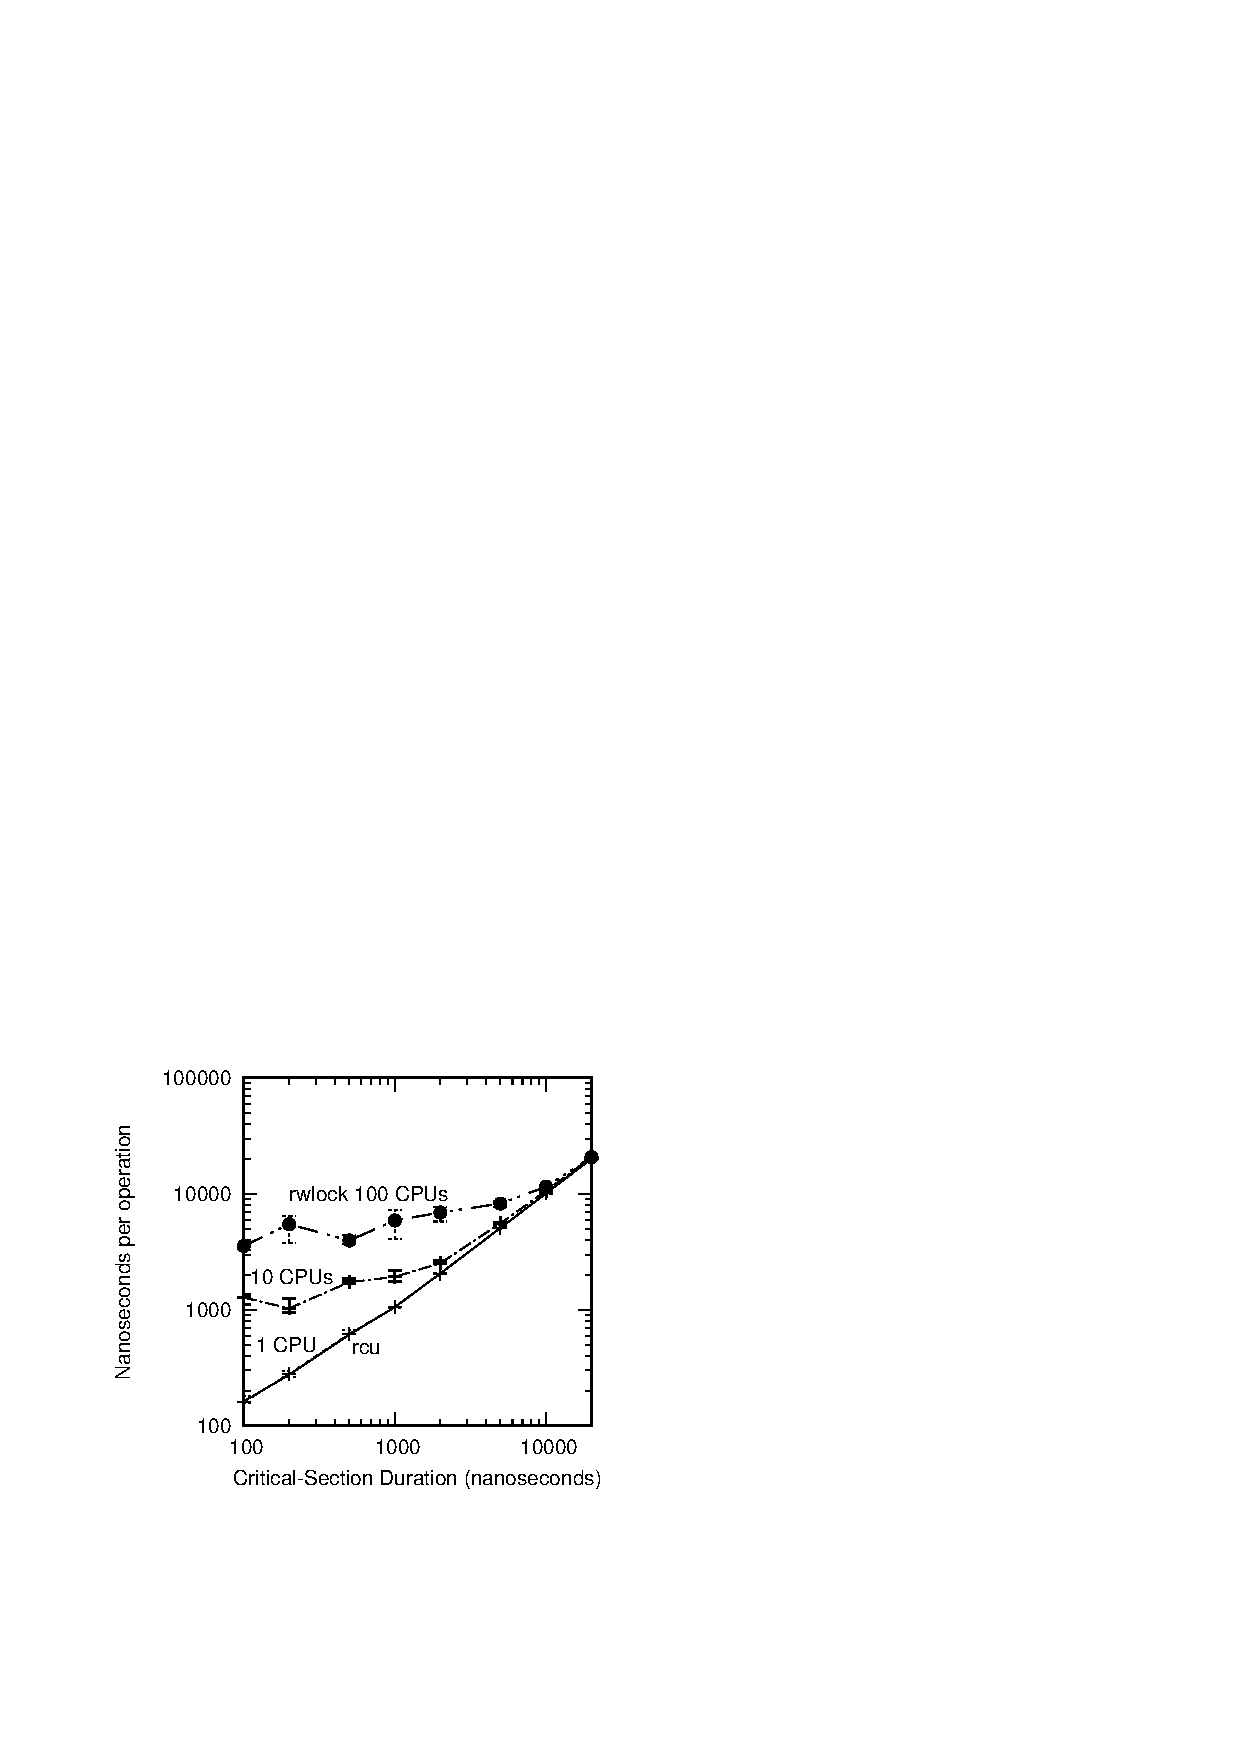
\includegraphics{CodeSamples/defer/data/rcuscale.hps.2020.05.28a/rwlockRCUperfwt}}
\caption{Comparison of RCU to Reader-Writer Locking as Function of Critical-Section Duration, 192 CPUs}
\label{fig:defer:Comparison of RCU to Reader-Writer Locking as Function of Critical-Section Duration}
\end{figure}

Of course, the low performance of reader-writer locking in
\cref{fig:defer:Performance Advantage of RCU Over Reader-Writer Locking,%
fig:defer:Performance Advantage of Preemptible RCU Over Reader-Writer Locking}
is exaggerated by the unrealistic zero-length critical sections.
The performance advantages of RCU decrease as the overhead of the critical
sections increase, as shown in
\cref{fig:defer:Comparison of RCU to Reader-Writer Locking as Function of Critical-Section Duration},
which was run on the same system as the previous plots.
Here, the y-axis represents the sum of the overhead of the read-side
primitives and that of the critical section and the x-axis represents
the critical-section overhead in nanoseconds.
But please note the logscale y~axis, which means that the small
separations between the traces still represent significant differences.
This figure shows non-preemptible RCU, but given that preemptible RCU's
read-side overhead is only about three nanoseconds, its plot would be
nearly identical to
\cref{fig:defer:Comparison of RCU to Reader-Writer Locking as Function of Critical-Section Duration}.

\QuickQuiz{
	Why the larger error ranges for the submicrosecond durations in
	\cref{fig:defer:Comparison of RCU to Reader-Writer Locking as Function of Critical-Section Duration}?
}\QuickQuizAnswer{
	Because smaller disturbances result in greater relative errors
	for smaller measurements.
	Also, the Linux kernel's \co{ndelay()} nanosecond-scale primitive
	is (as of 2020) less accurate than is the \co{udelay()} primitive
	used for the data for durations of a microsecond or more.
	It is instructive to compare to the zero-length case shown in
	\cref{fig:defer:Performance Advantage of RCU Over Reader-Writer Locking}.
}\QuickQuizEnd

There are three traces for reader-writer locking, with the upper trace
being for 100~CPUs, the next for 10~CPUs, and the lowest for 1~CPU\@.
The greater the number of CPUs and the shorter the critical sections,
the greater is RCU's performance advantage.
These performance advantages are underscored by the fact that 100-CPU
systems are no longer uncommon and that a number of system calls (and
thus any RCU read-side critical sections that they contain) complete
within microseconds.

In addition, as is discussed in the next paragraph,
RCU read-side primitives are almost entirely deadlock-immune.


\paragraph{Deadlock Immunity}

Although RCU offers significant performance advantages for
read-mostly workloads, one of the primary reasons for creating
RCU in the first place was in fact its immunity to read-side
deadlocks.
This immunity stems from the fact that
RCU read-side primitives do not block, spin, or even
do backwards branches, so that their execution time is deterministic.
It is therefore impossible for them to participate in a deadlock
cycle.

\QuickQuiz{
	Is there an exception to this deadlock immunity, and if so,
	what sequence of events could lead to deadlock?
}\QuickQuizAnswer{
	One way to cause a deadlock cycle involving
	RCU read-side primitives is via the following (illegal) sequence
	of statements:

\begin{VerbatimU}
rcu_read_lock();
synchronize_rcu();
rcu_read_unlock();
\end{VerbatimU}

	The \co{synchronize_rcu()} cannot return until all
	pre-existing RCU read-side critical sections complete, but
	is enclosed in an RCU read-side critical section that cannot
	complete until the \co{synchronize_rcu()} returns.
	The result is a classic self-deadlock---you get the same
	effect when attempting to write-acquire a reader-writer lock
	while read-holding it.

	Note that this self-deadlock scenario does not apply to
	RCU QSBR, because the context switch performed by the
	\co{synchronize_rcu()} would act as a quiescent state
	for this CPU, allowing a grace period to complete.
	However, this is if anything even worse, because data used
	by the RCU read-side critical section might be freed as a
	result of the grace period completing.
	Plus Linux kernel's lockdep facility will yell at you.

	In short, do not invoke synchronous RCU update-side primitives, which
	are listed in
	\cref{tab:defer:RCU Wait-to-Finish APIs},
	from within an RCU read-side critical section.

	In addition, within the Linux kernel, RCU uses the scheduler
	and the scheduler uses RCU\@.
	In some cases, both RCU and the scheduler must take care to
	avoid deadlock.
}\QuickQuizEnd

An interesting consequence of RCU's read-side deadlock immunity is
that it is possible to unconditionally upgrade an RCU
reader to an RCU updater.
Attempting to do such an upgrade with reader-writer locking results
in deadlock.
A sample code fragment that does an RCU read-to-update upgrade follows:

\begin{VerbatimN}[samepage=true]
rcu_read_lock();
list_for_each_entry_rcu(p, &head, list_field) {
	do_something_with(p);
	if (need_update(p)) {
		spin_lock(my_lock);
		do_update(p);
		spin_unlock(&my_lock);
	}
}
rcu_read_unlock();
\end{VerbatimN}

Note that \co{do_update()} is executed under
the protection of the lock \emph{and} under RCU read-side protection.

Another interesting consequence of RCU's deadlock immunity is its
immunity to a large class of priority inversion problems.
For example, low-priority RCU readers cannot prevent a high-priority
RCU updater from acquiring the update-side lock.
Similarly, a low-priority RCU updater cannot prevent high-priority
RCU readers from entering an RCU read-side critical section.

\QuickQuiz{
	Immunity to both deadlock and priority inversion???
	Sounds too good to be true.
	Why should I believe that this is even possible?
}\QuickQuizAnswer{
	It really does work.
	After all, if it didn't work, the Linux kernel would not run.
}\QuickQuizEnd

\paragraph{Realtime Latency}

Because RCU read-side primitives neither spin nor block, they offer
excellent realtime latencies.
In addition, as noted earlier, this means that they are
immune to priority inversion
involving the RCU read-side primitives and locks.

However, RCU is susceptible to more subtle priority-inversion scenarios,
for example, a high-priority process blocked waiting for an RCU
grace period to elapse can be blocked by low-priority RCU readers
in \rt\ kernels.
This can be solved by using RCU priority
boosting~\cite{PaulEMcKenney2007BoostRCU,DinakarGuniguntala2008IBMSysJ}.

However, use of RCU priority boosting requires that \co{rcu_read_unlock()}
do deboosting, which entails acquiring scheduler locks.
Some care is therefore required within the scheduler and RCU to avoid
deadlocks, which as of the v5.15 Linux kernel requires RCU to avoid
invoking the scheduler while holding any of RCU's locks.

This in turn means that \co{rcu_read_unlock()} is not always lockless
when RCU priority boosting is enabled.
However, \co{rcu_read_unlock()} will still be lockless if its
critical section was not priority-boosted.
Furthermore, critical sections will not be priority boosted unless they
are preempted, or, in -rt kernels, they acquire non-raw spinlocks.
This means that \co{rcu_read_unlock()} will normally be lockless from the
perspective of the highest priority task running on any given CPU.

\paragraph{RCU Readers and Updaters Run Concurrently}

Because RCU readers never spin nor block, and because updaters are not
subject to any sort of rollback or abort semantics, RCU readers and
updaters really can run concurrently.
This means that RCU readers might access stale data, and might even
see inconsistencies, either of which can render conversion from reader-writer
locking to RCU non-trivial.

\begin{figure}
\centering
\resizebox{3in}{!}{\includegraphics{defer/rwlockRCUupdate}}
\caption{Response Time of RCU vs.\@ Reader-Writer Locking}
\label{fig:defer:Response Time of RCU vs. Reader-Writer Locking}
\end{figure}

However, in a surprisingly large number of situations, inconsistencies and
stale data are not problems.
The classic example is the networking routing table.
Because routing updates can take considerable time to reach a given
system (seconds or even minutes), the system will have been sending
packets the wrong way for quite some time when the update arrives.
It is usually not a problem to continue sending updates the wrong
way for a few additional milliseconds.
Furthermore, because RCU updaters can make changes without waiting for
RCU readers to finish,
the RCU readers might well see the change more quickly than would
batch-fair
reader-writer-locking readers, as shown in
\cref{fig:defer:Response Time of RCU vs. Reader-Writer Locking}.

\QuickQuiz{
	But how many other algorithms really tolerate stale and
	inconsistent data?
}\QuickQuizAnswer{
	Quite a few!

	Please keep in mind that the finite speed of light means that
	data reaching a given computer system is at least slightly stale
	at the time that it arrives, and extremely stale in the case
	of astronomical data.
	The finite speed of light also places a sharp limit on the
	consistency of data arriving from different sources of via
	different paths.

	You might as well face the fact that the laws of physics
	are incompatible with naive notions of perfect freshness and
	consistency.
}\QuickQuizEnd

Once the update is received, the rwlock writer cannot proceed until the
last reader completes, and subsequent readers cannot proceed until the
writer completes.
However, these subsequent readers are guaranteed to see the new value,
as indicated by the green shading of the rightmost boxes.
In contrast, RCU readers and updaters do not block each other, which permits
the RCU readers to see the updated values sooner.
Of course, because their execution overlaps that of the RCU updater,
\emph{all} of the RCU readers might well see updated values, including
the three readers that started before the update.
Nevertheless only the green-shaded rightmost RCU readers
are \emph{guaranteed} to see the updated values.

Reader-writer locking and RCU simply provide different guarantees.
With reader-writer locking, any reader that begins after the writer begins
is guaranteed to see new values, and any reader that attempts to
begin while the writer is spinning might or might not see new values,
depending on the reader/writer preference of the rwlock implementation in
question.
In contrast, with RCU, any reader that begins after the updater completes
is guaranteed to see new values, and any reader that completes after the
updater begins might or might not see new values, depending on timing.

The key point here is that, although reader-writer locking does
indeed guarantee consistency within the confines of the computer system,
there are situations where this consistency comes at the price of
increased \emph{inconsistency} with the outside world, courtesy of
the finite speed of light and the non-zero size of atoms.
In other words, reader-writer locking obtains internal consistency at the
price of silently stale data with respect to the outside world.

Note that if a value is computed while read-holding a reader-writer
lock, and then that value is used after that lock is released, then
this reader-writer-locking use case is using stale data.
After all, the quantities that this value is based on could change
at any time after that lock is released.
This sort of reader-writer-locking use case is often easy to
convert to RCU, as will be shown in
\cref{lst:defer:Converting Reader-Writer Locking to RCU: Data,%
lst:defer:Converting Reader-Writer Locking to RCU: Search,%
lst:defer:Converting Reader-Writer Locking to RCU: Deletion}
and the accompanying text.

\paragraph{Low-Priority RCU Readers Can Block High-Priority Reclaimers}

In Realtime RCU~\cite{DinakarGuniguntala2008IBMSysJ} or
SRCU~\cite{PaulEMcKenney2006c},
a preempted reader will prevent a grace period from completing, even if
a high-priority task is blocked waiting for that grace period to complete.
Realtime RCU can avoid this problem by substituting \co{call_rcu()}
for \co{synchronize_rcu()} or by using RCU priority
boosting~\cite{PaulEMcKenney2007BoostRCU,DinakarGuniguntala2008IBMSysJ}.
It might someday be necessary to augment SRCU and RCU Tasks Trace with
priority boosting, but not before a clear real-world need is demonstrated.

\QuickQuiz{
	If Tasks RCU Trace might someday be priority boosted, why
	not also Tasks RCU and Tasks RCU Rude?
}\QuickQuizAnswer{
	Maybe, but these are less likely.

	In the case of Tasks RCU, recall that the quiescent state is
	a voluntary context switch.
	Thus, all tasks not blocked after a voluntary context switch
	might need to be boosted, and the mechanics of deboosting would
	not likely be at all pretty.

	In the case of Tasks RCU Rude, as was the case with the old
	RCU Sched, any preemptible region of code is a quiescent state.
	Thus, the only tasks that might need boosting are those currently
	running with preemption disabled.
	But boosting the priority of a preemption-disabled task has no
	effect.
	It therefore seems doubly unlikely that priority boosting will
	ever be introduced to Tasks RCU Rude, at least in its current
	form.
}\QuickQuizEnd

\paragraph{RCU Grace Periods Extend for Many Milliseconds}

With the exception of userspace
RCU~\cite{MathieuDesnoyers2009URCU,PaulMcKenney2013LWNURCU},
expedited grace periods, and several of the ``toy''
RCU implementations described in
\cref{chp:app:``Toy'' RCU Implementations},
RCU grace periods extend milliseconds.
Although there are a number of techniques to render such long
delays harmless, including use of the asynchronous interfaces
(\co{call_rcu()} and \co{call_rcu_bh()}) or of the polling interfaces
(\co{get_state_synchronize_rcu()}, \co{start_poll_synchronize_rcu()},
and \co{poll_state_synchronize_rcu()}), this situation is a major reason
for the rule of thumb that RCU be used in read-mostly situations.

As noted in \cref{sec:defer:RCU Linux-Kernel API}, within the Linux
kernel, shorter grace periods may be obtained via expedited grace
periods, for example, by invoking \co{synchronize_rcu_expedited()}
instead of \co{synchronize_rcu()}.
Expedited grace periods can reduce delays to as little as a few tens of
microseconds, albeit at the expense of higher CPU utilization and IPIs.
The added IPIs can be especially unwelcome in some real-time workloads.

\paragraph{Code:
		 Reader-Writer Locking vs.\@ RCU}

In the best case, the conversion from reader-writer locking to RCU
is quite simple, as shown in
\cref{lst:defer:Converting Reader-Writer Locking to RCU: Data,%
lst:defer:Converting Reader-Writer Locking to RCU: Search,%
lst:defer:Converting Reader-Writer Locking to RCU: Deletion},
all taken from
Wikipedia~\cite{WikipediaRCU}.

\begin{listing*}
{ \scriptsize
\begin{verbbox}
 1 struct el {                           1 struct el {
 2   struct list_head lp;                2   struct list_head lp;
 3   long key;                           3   long key;
 4   spinlock_t mutex;                   4   spinlock_t mutex;
 5   int data;                           5   int data;
 6   /* Other data fields */             6   /* Other data fields */
 7 };                                    7 };
 8 DEFINE_RWLOCK(listmutex);             8 DEFINE_SPINLOCK(listmutex);
 9 LIST_HEAD(head);                      9 LIST_HEAD(head);
\end{verbbox}
}
\hspace*{0.9in}\OneColumnHSpace{-0.5in}
\IfEbookSize{\hspace*{-1.05in}}{}\theverbbox
\caption{Converting Reader-Writer Locking to RCU\@:
						    Data}
\label{lst:defer:Converting Reader-Writer Locking to RCU: Data}
\end{listing*}

\begin{listing*}
{ \scriptsize
\begin{verbbox}
 1 int search(long key, int *result)     1 int search(long key, int *result)
 2 {                                     2 {
 3   struct el *p;                       3   struct el *p;
 4                                       4
 5   read_lock(&listmutex);              5   rcu_read_lock();
 6   list_for_each_entry(p, &head, lp) { 6   list_for_each_entry_rcu(p, &head, lp) {
 7     if (p->key == key) {              7     if (p->key == key) {
 8       *result = p->data;              8       *result = p->data;
 9       read_unlock(&listmutex);        9       rcu_read_unlock();
10       return 1;                      10       return 1;
11     }                                11     }
12   }                                  12   }
13   read_unlock(&listmutex);           13   rcu_read_unlock();
14   return 0;                          14   return 0;
15 }                                    15 }
\end{verbbox}
}
\hspace*{0.9in}\OneColumnHSpace{-0.5in}
\IfEbookSize{\hspace*{-1.05in}}{}\theverbbox
\caption{Converting Reader-Writer Locking to RCU\@:
						    Search}
\label{lst:defer:Converting Reader-Writer Locking to RCU: Search}
\end{listing*}

\begin{listing*}
{ \scriptsize
\begin{verbbox}
 1 int delete(long key)                  1 int delete(long key)
 2 {                                     2 {
 3   struct el *p;                       3   struct el *p;
 4                                       4
 5   write_lock(&listmutex);             5   spin_lock(&listmutex);
 6   list_for_each_entry(p, &head, lp) { 6   list_for_each_entry(p, &head, lp) {
 7     if (p->key == key) {              7     if (p->key == key) {
 8       list_del(&p->lp);               8       list_del_rcu(&p->lp);
 9       write_unlock(&listmutex);       9       spin_unlock(&listmutex);
                                        10       synchronize_rcu();
10       kfree(p);                      11       kfree(p);
11       return 1;                      12       return 1;
12     }                                13     }
13   }                                  14   }
14   write_unlock(&listmutex);          15   spin_unlock(&listmutex);
15   return 0;                          16   return 0;
16 }                                    17 }
\end{verbbox}
}
\hspace*{0.9in}\OneColumnHSpace{-0.5in}
\IfEbookSize{\hspace*{-1.05in}}{}\theverbbox
\caption{Converting Reader-Writer Locking to RCU\@:
						    Deletion}
\label{lst:defer:Converting Reader-Writer Locking to RCU: Deletion}
\end{listing*}

However, the transformation is not always this straightforward.
This is because neither the \co{spin_lock()} nor the
\co{synchronize_rcu()} in
\cref{lst:defer:Converting Reader-Writer Locking to RCU: Deletion}
exclude the readers in
\cref{lst:defer:Converting Reader-Writer Locking to RCU: Search}.
First, the \co{spin_lock()} does not interact in any way with
\co{rcu_read_lock()} and \co{rcu_read_unlock()}, thus not excluding them.
Second, although both \co{write_lock()} and \co{synchronize_rcu()}
wait for pre-existing readers, only \co{write_lock()} prevents
subsequent readers from commencing.\footnote{
	Kudos to whoever pointed this out to Paul.}
Thus, \co{synchronize_rcu()} cannot exclude readers.
Nevertheless, a great many situations using reader-writer locking can
be converted to RCU\@.

More-elaborate cases of replacing reader-writer locking with RCU
may be found
elsewhere~\cite{NeilBrown2015PathnameLookup,NeilBrown2015RCUwalk}.

\paragraph{Semantics:
		      Reader-Writer Locking vs.\@ RCU}

Expanding on the previous section, reader-writer locking semantics can
be roughly and informally summarized by the following three temporal
constraints:

\begin{enumerate}
\item	Write-side acquisitions wait for any read-holders to release
	the lock.
\item	Writer-side acquisitions wait for any write-holder to release
	the lock.
\item	Read-side acquisitions wait for any write-holder to release
	the lock.
\end{enumerate}

RCU dispenses entirely with constraint~\#3 and weakens the other two
as follows:

\begin{enumerate}
\item	Writers wait for any pre-existing read-holders before progressing
	to the destructive phase of their update (usually the freeing of
	memory).
\item	Writers synchronize with each other as needed.
\end{enumerate}

It is of course this weakening that permits RCU implementations to attain
excellent performance and scalability.
It also allows RCU to implement the aforementioned unconditional
read-to-write upgrade that is so attractive and so deadlock-prone in
reader-writer locking.
Code using RCU can compensate for this weakening in a surprisingly large
number of ways, but most commonly by imposing spatial constraints:

\begin{enumerate}
\item	New data is placed in newly allocated memory.
\item	Old data is freed, but only after:
	\begin{enumerate}
	\item	That data has been unlinked so as to be inaccessible
		to later readers, and
	\item	A subsequent RCU grace period has elapsed.
	\end{enumerate}
\end{enumerate}

Of course, there are some reader-writer-locking use cases for which
RCU's weakened semantics are inappropriate, but experience in the Linux
kernel indicates that more than 80\% of reader-writer locks can in fact
be replaced by RCU\@.
For example, a common reader-writer-locking use case computes some value
while holding the lock and then uses that value after releasing that lock.
This use case results in stale data, and therefore often accommodates
RCU's weaker semantics.

\begin{listing}
\input{CodeSamples/defer/singleton@get.fcv}
\caption{RCU Singleton Get}
\label{lst:defer:Singleton Get}
\end{listing}

\begin{listing}
\input{CodeSamples/defer/singleton@set.fcv}
\caption{RCU Singleton Set}
\label{lst:defer:Singleton Set}
\end{listing}

\begin{fcvref}[ln:defer:singleton:get]
This interaction of temporal and spatial constraints is illustrated
by the RCU singleton data structure illustrated in
\cref{fig:defer:Insertion With Concurrent Readers,fig:defer:Deletion With Concurrent Readers}.
This structure is defined on \clnrefrange{myconfig.b}{myconfig.e} of
\cref{lst:defer:Singleton Get}, and contains two integer fields,
\co{->a} and \co{->b} (\path{singleton.c}).
The current instance of this structure is referenced by the \co{curconfig}
pointer defined on \clnref{myconfig.e}.
\end{fcvref}

\begin{fcvref}[ln:defer:singleton:get]
The fields of the current structure are passed back through the
\co{cur_a} and \co{cur_b} parameters to the \co{get_config()} function
defined on \clnrefrange{get_config.b}{get_config.e}.
These two fields can be slightly out of date, but they absolutely must
be consistent with each other.
The \co{get_config()} function provides this consistency
within the RCU read-side critical section starting on
\clnref{rrl} and ending on either \clnref{rrul1} or \clnref{rrul2},
which provides the needed temporal synchronization.
\Clnref{rderef} fetches the pointer to the current \co{myconfig} structure.
This structure will be used regardless of any concurrent changes due
to calls to the \co{set_config()} function, thus providing the needed
spatial synchronization.
If \clnref{nullchk} determines that the \co{curconfig} pointer was
\co{NULL}, \clnref{retfail} returns failure.
Otherwise, \clnref{copya,copyb} copy out the \co{->a} and \co{->b} fields
and \clnref{retsuccess} returns success.
These \co{->a} and \co{->b} fields are from the same \co{myconfig}
structure, and the RCU read-side critical section prevents this structure
from being freed, thus guaranteeing that these two fields are consistent
with each other.
\end{fcvref}

\begin{fcvref}[ln:defer:singleton:set]
The structure is updated by the \co{set_config()} function shown in
\cref{lst:defer:Singleton Set}.
\Clnrefrange{allocinit.b}{allocinit.e} allocate and initialize a
new \co{myconfig} structure.
\Clnref{xchg} atomically exchanges a pointer to this new structure with
the pointer to the old structure in \co{curconfig}, while also providing
full memory ordering both before and after the \co{xchg()} operation,
thus providing the needed updater/reader spatial synchronization on
the one hand and the needed updater/updater synchronization on the other.
If \clnref{if} determines that the pointer to the old structure was
in fact non-\co{NULL}, \clnref{sr} waits for a grace period (thus providing
the needed reader/updater temporal synchronization) and \clnref{free}
frees the old structure, safe in the knowledge that there are no
longer any readers still referencing it.
\end{fcvref}

\begin{figure*}
\centering
\resizebox{\onecolumntextwidth}{!}{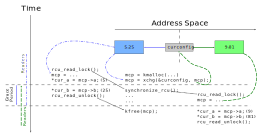
\includegraphics{defer/RCUspacetime}}
\caption{RCU Spatial/Temporal Synchronization}
\label{fig:defer:RCU Spatial/Temporal Synchronization}
\end{figure*}

\Cref{fig:defer:RCU Spatial/Temporal Synchronization} shows an abbreviated
representation of \co{get_config()} on the left and right and a similarly
abbreviated representation of \co{set_config()} in the middle.
Time advances from top to bottom, and the address space of the objects
referenced by \co{curconfig} advances from left to right.
The boxes with comma-separated numbers each represent a \co{myconfig}
structure, with the constraint that \co{->b} is the square of \co{->a}.
Each blue dash-dotted arrow represents an interaction with the old structure
(on the left, containing ``5,25'') and each green dashed arrow represents
an interaction with the new structure (on the right, containing ``9,81'').

The black dotted arrows represent temporal relationships between RCU readers
on the left and right and the RCU grace period at center, with each
arrow pointing from an older event to a newer event.
The call to \co{synchronize_rcu()} followed the leftmost \co{rcu_read_lock()},
and therefore that \co{synchronize_rcu()} invocation must not return
until after the corresponding \co{rcu_read_unlock()}.
In contrast, the call to \co{synchronize_rcu()} precedes the
rightmost \co{rcu_read_lock()}, which allows the return from that same
\co{synchronize_rcu()} to ignore the corresponding \co{rcu_read_unlock()}.
These temporal relationships prevent the \co{myconfig} structures from
being freed while RCU readers are still accessing them.

The two horizontal grey dashed lines represent the period of time during
which different readers get different results, however, each reader
will see one and only one of the two objects.
All readers that end before the first horizontal line will see the
leftmost \co{myconfig} structure, and all readers that start after the
second horizontal line will see the rightmost structure.
Between the two lines, that is, during the grace period, different
readers might see different objects, but as long as each reader
loads the \co{curconfig} pointer only once, each reader will see
a consistent view of its \co{myconfig} structure.

\QuickQuiz{
	But doesn't the RCU grace period start sometime after the
	call to \co{synchronize_rcu()} rather than in the middle
	of that \co{xchg()} statement?
}\QuickQuizAnswer{
	Which grace period, exactly?

	The updater is required to wait for at least one grace
	period that starts at or some time after the removal,
	in this case, the \co{xchg()}.
	So in
	\cref{fig:defer:RCU Spatial/Temporal Synchronization},
	the indicated grace period starts as early as theoretically
	possible and extends to the return from \co{synchronize_rcu()}.
	This is a perfectly legal grace period corresponding to the
	change carried out by that \co{xchg()} statement.
}\QuickQuizEnd

In short, when operating on a suitable linked data structure, RCU
combines temporal and spatial synchronization in order to approximate
reader-writer locking, with RCU read-side critical sections acting as
the reader-writer-locking reader, as shown in
\cref{fig:defer:Relationships Between RCU Use Cases,fig:defer:RCU Spatial/Temporal Synchronization}.
RCU's temporal synchronization is provided by the read-side markers,
for example, \co{rcu_read_lock()} and \co{rcu_read_unlock()}, as well as
the update-side grace-period primitives, for example, \co{synchronize_rcu()}
or \co{call_rcu()}.
The spatial synchronization is provided by the read-side
\co{rcu_dereference()} family of primitives, each of which subscribes
to a version published by \co{rcu_assign_pointer()}.\footnote{
	Preferably with both \co{rcu_dereference()} and
	\co{rcu_assign_pointer()} being embedded in higher-level APIs.}
RCU's combining of temporal and spatial synchronization contrasts to
the schemes presented in
\cref{sec:SMPdesign:Code Locking,sec:SMPdesign:Data Locking,sec:locking:Inefficiency},
in which temporal and spatial synchronization are provided separately by
locking and by static data-structure layout, respectively.

\QuickQuiz{
	Is RCU the only synchronization mechanism that combines temporal
	and spatial synchronization in this way?
}\QuickQuizAnswer{
	Not at all.

	Hazard pointers can be considered to combine temporal and spatial
	synchronization in a similar manner.
	Referring to
	\cref{lst:defer:Hazard-Pointer Recording and Clearing},
	the \co{hp_record()} function's acquisition of a reference
	provides both spatial and temporal synchronization, subscribing
	to a version and marking the start of a reference, respectively.
	This function therefore combines the effects of RCU's
	\co{rcu_read_lock()} and \co{rcu_dereference()}.
	Referring now to
	\cref{lst:defer:Hazard-Pointer Scanning and Freeing},
	the \co{hp_clear()} function's release of a reference provides
	temporal synchronization marking the end of a reference, and is
	thus similar to RCU's \co{rcu_read_unlock()}.
	The \co{hazptr_free_later()} function's retiring of a
	hazard-pointer-protected object provides temporal synchronization,
	similar to RCU's \co{call_rcu()}.
	The primitives used to mutate a hazard-pointer-protected
	structure provide spatial synchronization, similar to RCU's
	\co{rcu_assign_pointer()}.

	Alternatively, one could instead come at hazard pointers by
	analogy with reference counting.
}\QuickQuizEnd

\subsubsection{Quasi Reference Count}
\label{sec:defer:Quasi Reference Count}

Because grace periods are not allowed to complete while
there is an RCU read-side critical section in progress,
the RCU read-side primitives may be used as a restricted
reference-counting mechanism.
For example, consider the following code fragment:

\begin{VerbatimN}
rcu_read_lock();  /* acquire reference. */
p = rcu_dereference(head);
/* do something with p. */
rcu_read_unlock();  /* release reference. */
\end{VerbatimN}

The combination of the \co{rcu_read_lock()} and \co{rcu_dereference()}
primitives can be thought of as acquiring a reference to \co{p},
because a grace period starting after the \co{rcu_dereference()}
assignment to \co{p} cannot possibly end until after we reach the matching
\co{rcu_read_unlock()}.
This reference-counting scheme is restricted in that it is forbidden
to wait for RCU grace periods within RCU read-side critical sections,
and also forbidden to hand off an RCU read-side critical section's
references from one task to another.

Regardless of these restrictions,
the following code can safely delete \co{p}:

\begin{VerbatimN}
spin_lock(&mylock);
p = head;
rcu_assign_pointer(head, NULL);
spin_unlock(&mylock);
/* Wait for all references to be released. */
synchronize_rcu();
kfree(p);
\end{VerbatimN}

The assignment to \co{head} prevents any future references
to \co{p} from being acquired, and the \co{synchronize_rcu()}
waits for any previously acquired references to be released.

\QuickQuiz{
	But wait!
	This is exactly the same code that might be used when thinking
	of RCU as a replacement for reader-writer locking!
	What gives?
}\QuickQuizAnswer{
	This is an effect of the Law of Toy Examples:
	Beyond a certain point, the code fragments look the same.
	The only difference is in how we think about the code.
	For example, what does an \co{atomic_inc()} operation do?
	It might be acquiring another explicit reference to an object
	to which we already have a reference, it might be incrementing
	an often-read/seldom-updated statistical counter, it might
	be checking into an HPC-style barrier, or any of a number of
	other things.

	However, these differences can be extremely important.
	For but one example of the importance, consider that if we think
	of RCU as a restricted reference counting scheme, we would never
	be fooled into thinking that the updates would exclude the RCU
	read-side critical sections.

	It nevertheless is often useful to think of RCU as a replacement
	for reader-writer locking, for example, when you are replacing
	reader-writer locking with RCU\@.
}\QuickQuizEnd

Of course, RCU can also be combined with traditional reference counting,
as discussed in
\cref{sec:together:Refurbish Reference Counting}.

\begin{figure}
\centering
\resizebox{2.5in}{!}{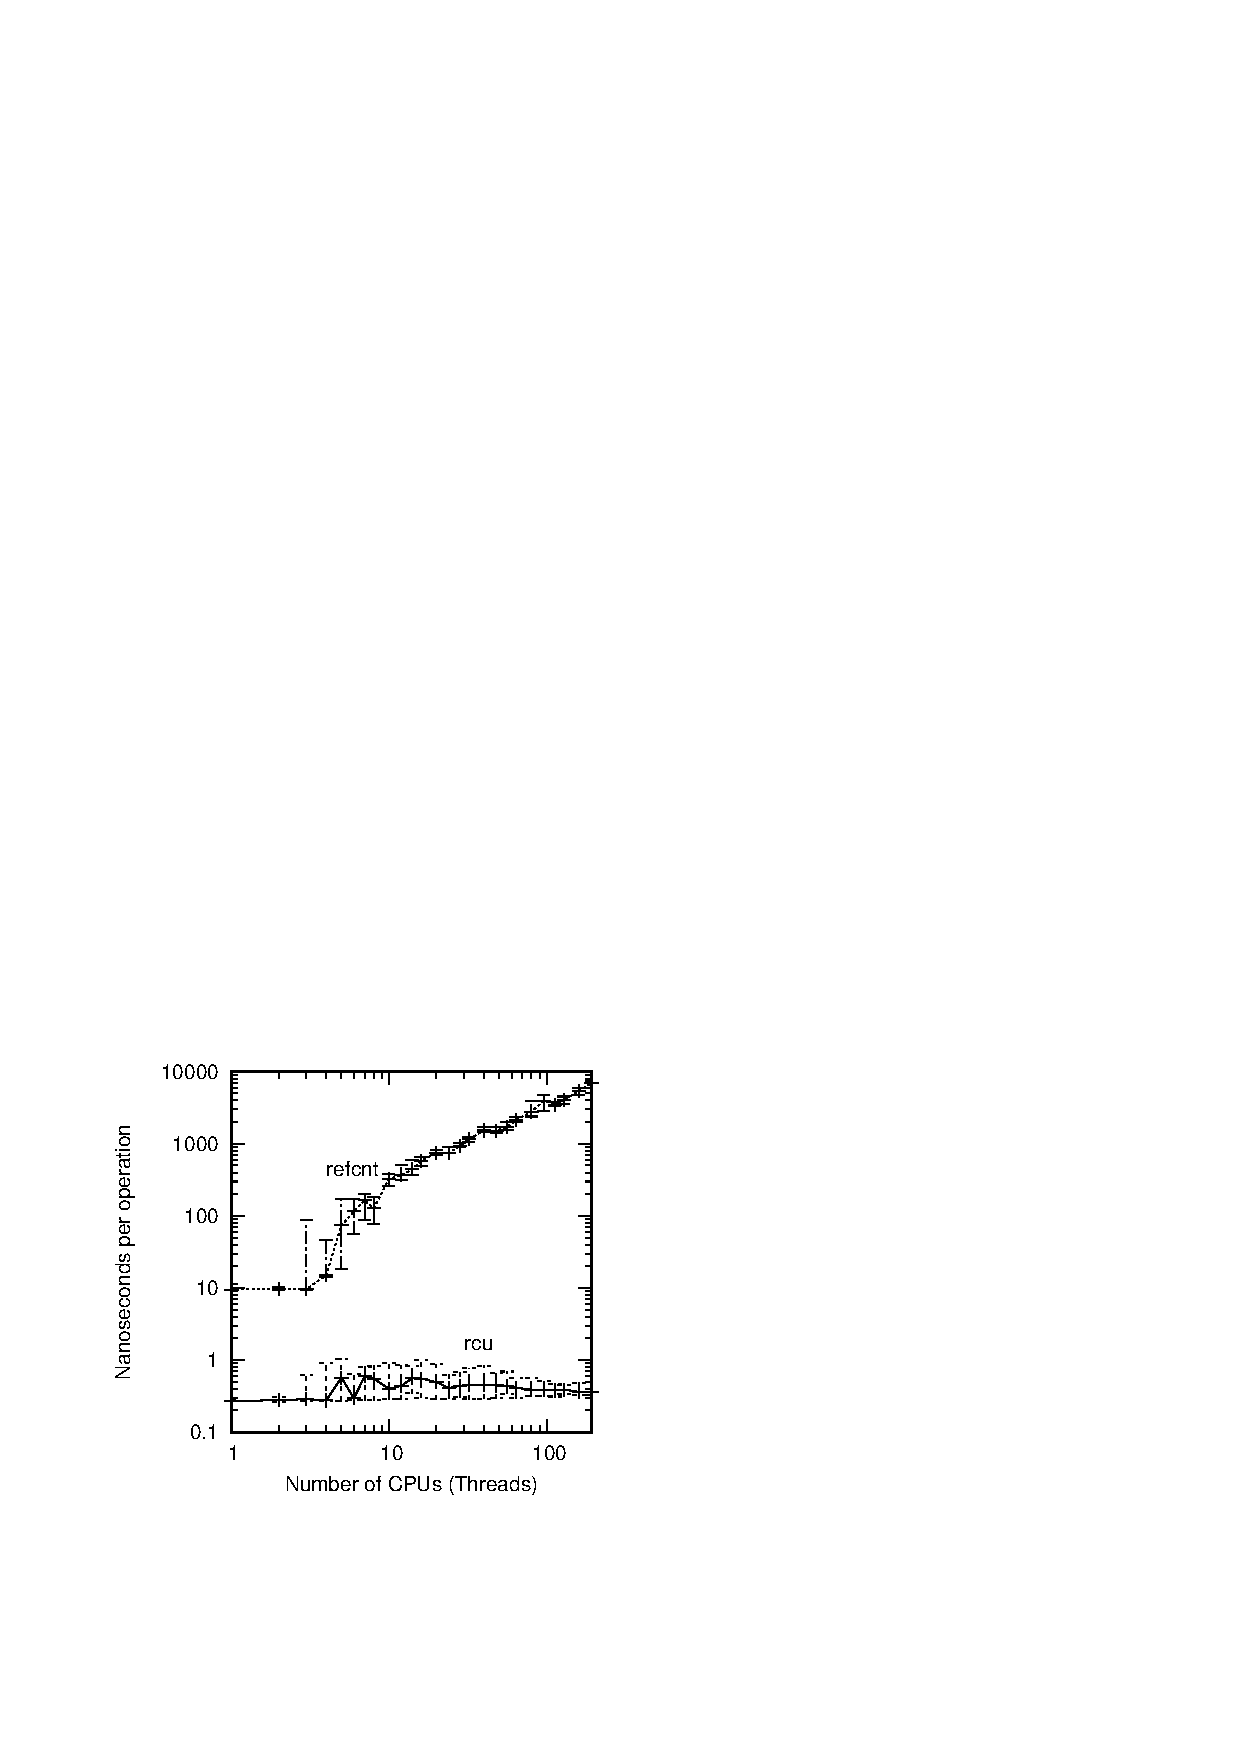
\includegraphics{CodeSamples/defer/data/rcuscale.hps.2020.05.28a/refcntRCUperf}}
\caption{Performance of RCU vs.\@ Reference Counting}
\label{fig:defer:Performance of RCU vs. Reference Counting}
\end{figure}

\begin{figure}
\centering
\resizebox{2.5in}{!}{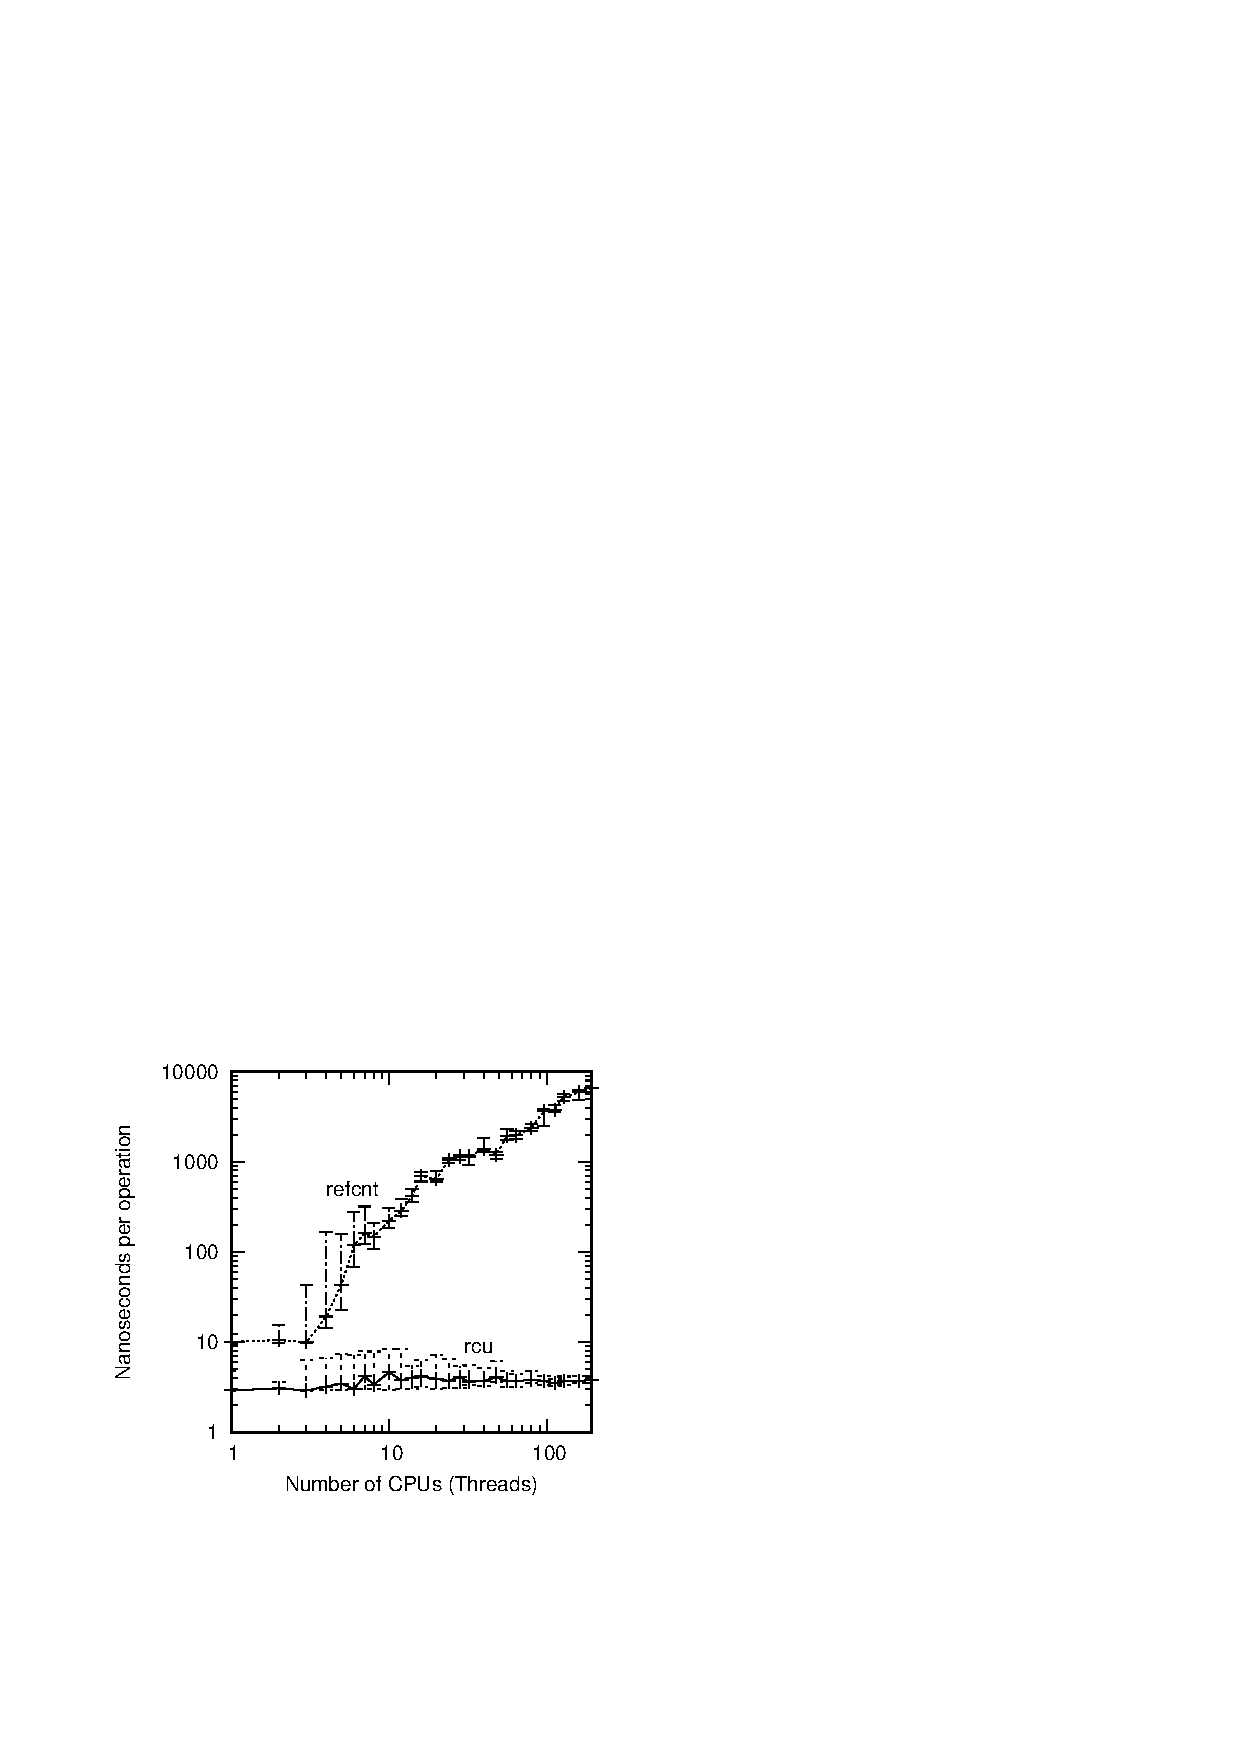
\includegraphics{CodeSamples/defer/data/rcuscale.hps.2020.05.28a/refRCUperfPREEMPT}}
\caption{Performance of Preemptible RCU vs.\@ Reference Counting}
\label{fig:defer:Performance of Preemptible RCU vs. Reference Counting}
\end{figure}

But why bother?
Again, part of the answer is performance, as shown in
\cref{fig:defer:Performance of RCU vs. Reference Counting,%
fig:defer:Performance of Preemptible RCU vs. Reference Counting},
again showing data taken on a 448-CPU 2.1\,GHz Intel x86 system
for non-preemptible and preemptible Linux-kernel RCU, respectively.
Non-preemptible RCU's advantage over
\IXalt{reference counting}{reference count} ranges from
more than an order of magnitude at one CPU up to about four orders of
magnitude at 192~CPUs.
Preemptible RCU's advantage ranges from about a factor of three at
one CPU up to about three orders of magnitude at 192~CPUs.

\begin{figure}
\centering
\resizebox{2.5in}{!}{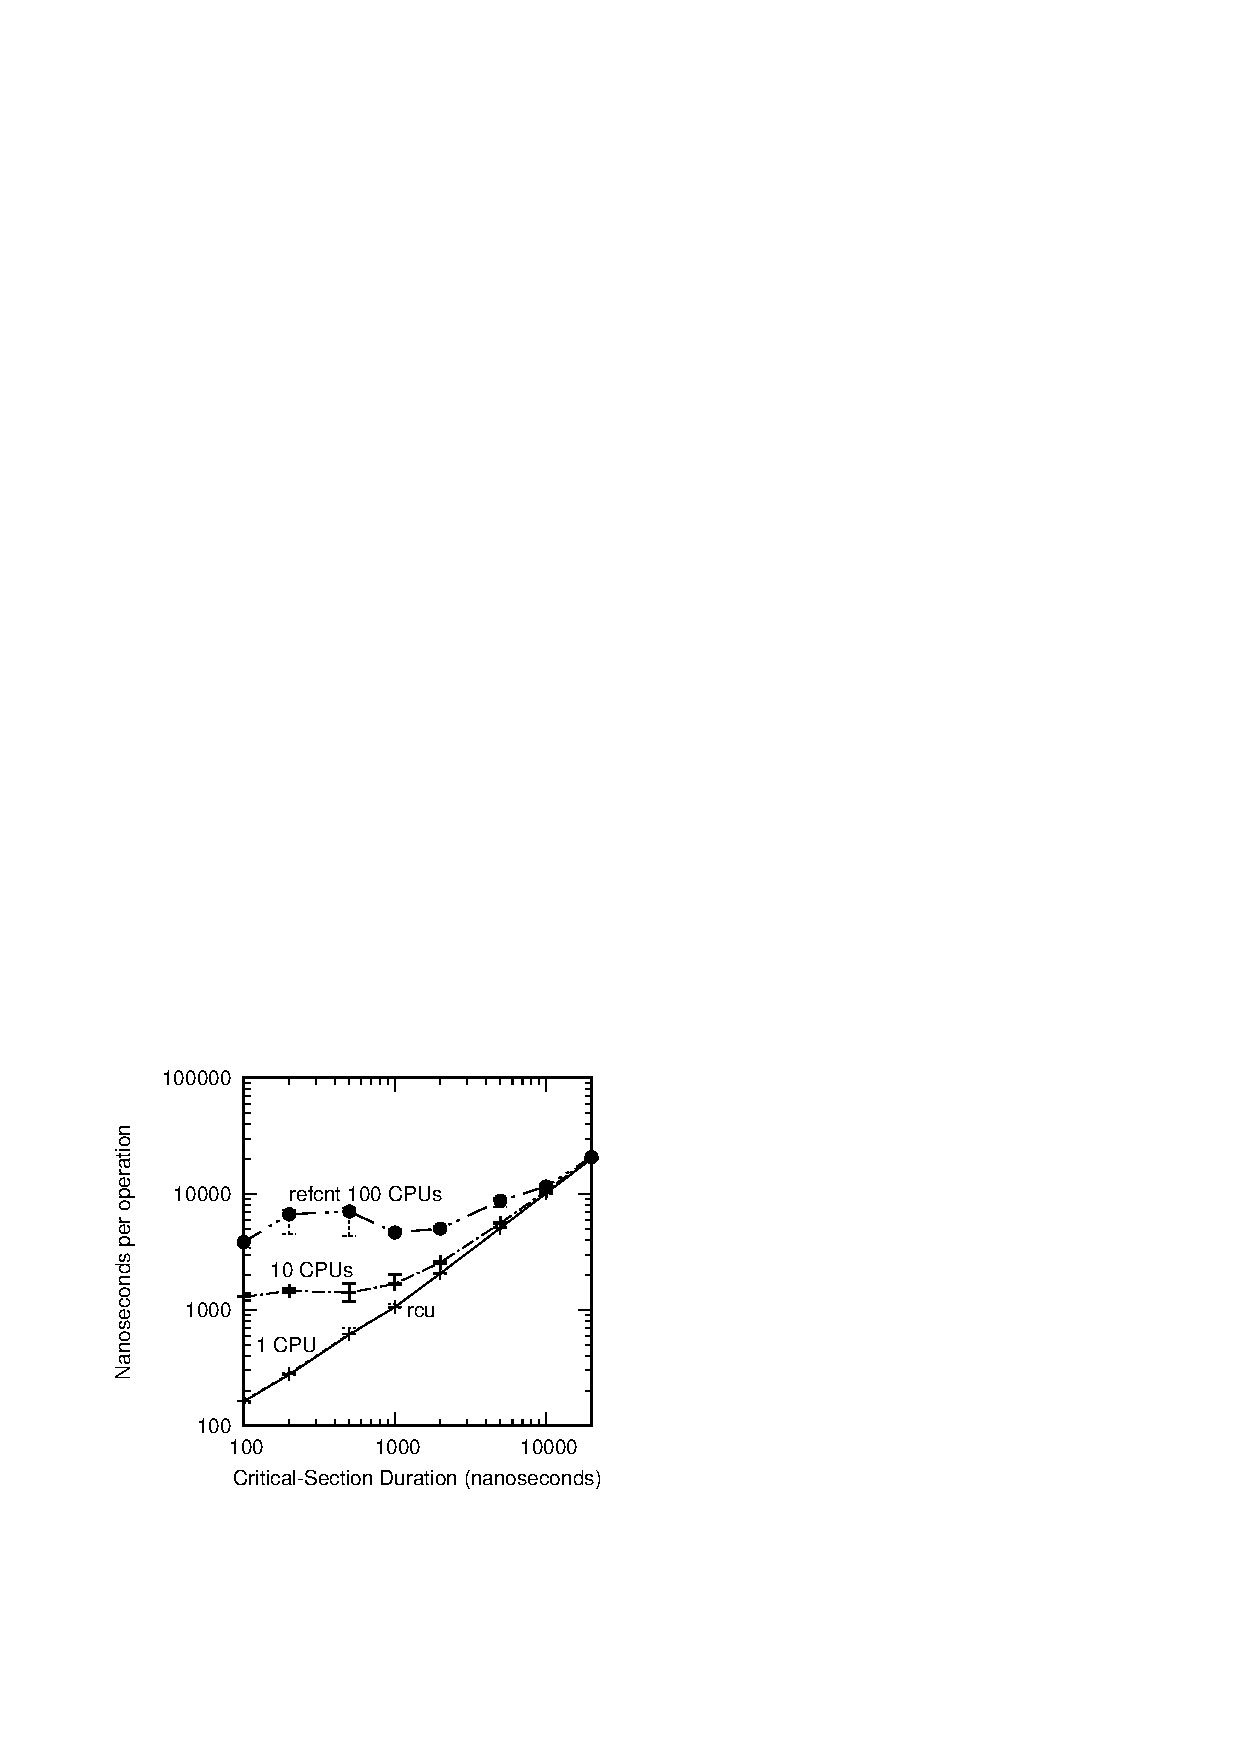
\includegraphics{CodeSamples/defer/data/rcuscale.hps.2020.05.28a/refRCUperfwt}}
\caption{Response Time of RCU vs.\@ Reference Counting, 192 CPUs}
\label{fig:defer:Response Time of RCU vs. Reference Counting}
\end{figure}

However, as with reader-writer locking, the performance advantages of
RCU are most pronounced for short-duration critical sections and for
large numbers of CPUs, as shown in
\cref{fig:defer:Response Time of RCU vs. Reference Counting}
for the same system.
In addition, as with reader-writer locking, many system calls (and thus
any RCU read-side critical sections that they contain) complete in
a few microseconds.

Although traditional reference counters are usually associated with a
specific data structure, or perhaps a specific group of data structures,
this approach does have some disadvantages.
For example, maintaining a single global reference counter for a large
variety of data structures typically results in bouncing the cache line
containing the reference count.
As we saw in
\crefrange{fig:defer:Performance of RCU vs. Reference Counting}{fig:defer:Response Time of RCU vs. Reference Counting},
such cache-line bouncing can severely degrade performance.

In contrast, RCU's lightweight \co{rcu_read_lock()},
\co{rcu_dereference()}, and \co{rcu_read_unlock()} read-side primitives
permit extremely frequent read-side usage with negligible performance
degradation.
Except that the calls to \co{rcu_dereference()} are not doing anything
specific to acquire a reference to the pointed-to object.
The heavy lifting is instead done by the \co{rcu_read_lock()} and
\co{rcu_read_unlock()} primitives and their interactions with RCU
grace periods.

And ignoring those calls to \co{rcu_dereference()} permits RCU to be
thought of as a ``bulk reference-counting'' mechanism, where each call
to \co{rcu_read_lock()} obtains a reference on each and every RCU-protected
object, and with little or no overhead.
However, the restrictions that go with RCU can be quite onerous.
For example, in many cases, the Linux-kernel prohibition against
sleeping while in an RCU read-side critical section would defeat the
entire purpose.
Such cases might be better served by the hazard pointers mechanism
described in \cref{sec:defer:Hazard Pointers}.
Cases where code rarely sleeps have been handled by using RCU as a
reference count in the common non-sleeping case and by bridging
to an explicit reference counter when sleeping is necessary.

Alternatively, situations where a reference must be held by a single task
across a section of code that sleeps may be accommodated with Sleepable
RCU (SRCU)~\cite{PaulEMcKenney2006c}.
This fails to cover the not-uncommon situation where a reference is ``passed''
from one task to another, for example, when a reference is acquired
when starting an I/O and released in the corresponding completion
interrupt handler.
Again, such cases might be better handled by explicit reference counters
or by hazard pointers.

Of course, SRCU brings restrictions of its own, namely that the
return value from \co{srcu_read_lock()} be passed into the
corresponding \co{srcu_read_unlock()}, and that no SRCU primitives
be invoked from hardware interrupt handlers or from \IXacrf{nmi}
handlers.
The jury is still out as to how much of a problem is presented by
this restriction, and as to how it can best be handled.

However, in the common case where references are held within the confines
of a single CPU or task, RCU can be used as high-performance and highly
scalable reference-counting mechanism.

As shown in \cref{fig:defer:Relationships Between RCU Use Cases},
quasi reference counts add RCU readers as individual or bulk
reference counts, possibly also bridging to reference counters
in corner cases.

\subsubsection{Quasi Multi-Version Concurrency Control}
\label{sec:defer:Quasi Multi-Version Concurrency Control}

RCU can also be thought of as a simplified multi-version concurrency
control (MVCC) mechanism with weak consistency criteria.
The multi-version aspects were touched upon in
\cref{sec:defer:Maintain Multiple Versions of Recently Updated Objects}.
However, in its native form, RCU provides version consistency only
within a given RCU-protected data element.

Nevertheless, there are situations where consistency and fresh data are
required across multiple data elements.
Fortunately, there are a number of approaches that avoid inconsistency
and stale data, including the following:

\begin{enumerate}
\item	Enclose RCU readers within sequence-locking readers, forcing
	the RCU readers to be retried should an update occur,
	as described in
	\cref{sec:together:Correlated Data Elements}
	and
	\cref{sec:together:Atomic Move}.
\item	Place the data that must be consistent into a single element
	of a linked data structure, and refrain from updating those
	fields within any element visible to RCU readers.
	RCU readers gaining a reference to any such element are then
	guaranteed to see consistent values.
	See \cref{sec:together:Correlated Fields} for additional details.
\item	Use a per-element lock that guards a ``deleted'' flag to allow
	RCU readers to reject stale
	data~\cite{PaulEdwardMcKenneyPhD,Arcangeli03}.
\item	Provide an existence flag that is referenced by all data elements
	whose update is to appear atomic to RCU
	readers~\cite{PaulEMcKennneyAtomicTreeN4037,PaulEMcKennneyAtomicTreeCPPCON2014,PaulEMcKenneyIssaquahUpdate2015,PaulEMcKenney2016IssaquahACMApp,PaulEMcKenney2016IssaquahCPPCON}.
\item	Use one of a wide range of counter-based
	methods~\cite{PaulEMcKenney2008cyclicRCU,PaulEMcKenney2010cyclicRCU,PaulEMcKenney2011cyclicparallelRCU,PaulEMcKenney2014cyclicRCU,Matveev:2015:RLS:2815400.2815406,Kim:2019:MSR:3297858.3304040}.
	In these approaches, updaters maintain a version number and maintain links
	to old versions of a given piece of data.
	Readers take a snapshot of the current version number, and, if necessary,
	traverse the links to find a version consistent with that snapshot.
\end{enumerate}

In short, when using RCU to approximate multi-version concurrency control,
you only pay for the level of consistency that you actually need.

As shown in \cref{fig:defer:Relationships Between RCU Use Cases},
quasi multi-version concurrency control is based on existence guarantees,
adding read-side snapshot operations and constraints on readers and
writers, the exact form of the constraint being dictated by the
consistency requirements, as summarized above.

\subsubsection{RCU Usage Summary}
\label{sec:defer:RCU Usage Summary}

At its core, RCU is nothing more nor less than an API that provides:

\begin{enumerate}
\item	A publish-subscribe mechanism for adding new data,
\item	A way of waiting for pre-existing RCU readers to finish, and
\item	A discipline of maintaining multiple versions to permit change
	without harming or unduly delaying concurrent RCU readers.
\end{enumerate}

That said, it is possible to build higher-level constructs on top of RCU,
including the various use cases described in the earlier sections.
Furthermore, I have no doubt that new use cases will continue to be
found for RCU, as well as for any of a number of other synchronization
primitives.
And so it is that RCU's use cases are conceptually more complex than
is RCU itself, as hinted on
\cpageref{sec:defer:Mysteries RCU Use Cases}.

\QuickQuiz{
	Which of these use cases best describes the Pre-BSD routing
	example in
	\cref{sec:defer:RCU for Pre-BSD Routing}?
}\QuickQuizAnswer{
	Pre-BSD routing could be argued to fit into either
	quasi reader-writer lock, quasi reference count, or
	quasi multi-version concurrency control.
	The code is the same either way.
	This is similar to things like \co{atomic_inc()}, another tool
	that can be put to a great many uses.
}\QuickQuizEnd

\begin{figure}
\centering
\resizebox{3in}{!}{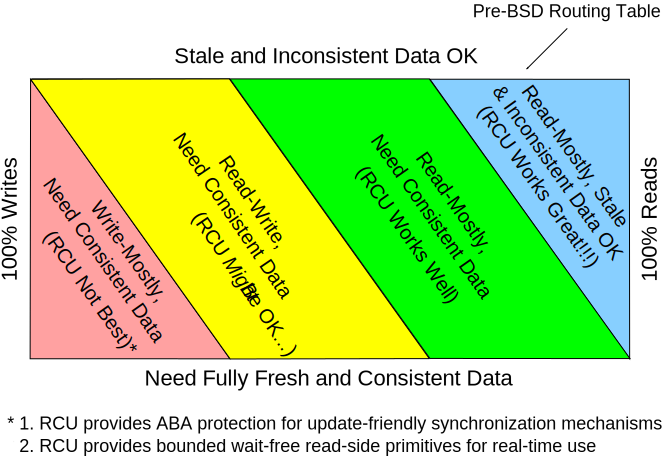
\includegraphics{defer/RCUApplicability}}
\caption{RCU Areas of Applicability}
\label{fig:defer:RCU Areas of Applicability}
\end{figure}

In the meantime,
\cref{fig:defer:RCU Areas of Applicability}
shows some rough rules of thumb on where RCU is most helpful.

As shown in the blue box in the upper-right corner of the figure, RCU
works best if you have read-mostly data where stale and inconsistent
data is permissible (but see below for more information on stale and
inconsistent data).
The canonical example of this case in the Linux kernel is routing tables.
Because it may have taken many seconds or even minutes for the
routing updates to propagate across the Internet, the system
has been sending packets the wrong way for quite some time.
Having some small probability of continuing to send some of them the wrong
way for a few more milliseconds is almost never a problem.

If you have a read-mostly workload where consistent data is required,
RCU works well, as shown by the green ``read-mostly, need consistent data''
box.
One example of this case is the Linux kernel's mapping from user-level
System-V semaphore IDs to the corresponding in-kernel data structures.
Semaphores tend to be used far more frequently than they are created
and destroyed, so this mapping is read-mostly.
However, it would be erroneous to perform a semaphore operation on
a semaphore that has already been deleted.
This need for consistency is handled by using the lock in the
in-kernel semaphore data structure, along with a ``deleted''
flag that is set when deleting a semaphore.
If a user ID maps to an in-kernel data structure with the
``deleted'' flag set, the data structure is ignored, so that
the user ID is flagged as invalid.

Although this requires that the readers acquire a lock for the
data structure representing the semaphore itself,
it allows them to dispense with locking for the
mapping data structure.
The readers therefore locklessly
traverse the tree used to map from ID to data structure,
which in turn greatly improves performance, scalability, and
real-time response.

As indicated by the yellow ``read-write'' box, RCU can also be useful
for read-write
workloads where consistent data is required, although usually in
conjunction with a number of other synchronization primitives.
For example, the directory-entry cache in recent Linux kernels uses RCU in
conjunction with sequence locks, per-CPU locks, and per-data-structure
locks to allow lockless traversal of pathnames in the common case.
Although RCU can be very beneficial in this read-write case, the
corresponding code is often more complex than that of the read-mostly
cases.

Finally, as indicated by the red box in the lower-left corner
of the figure, update-mostly workloads requiring consistent
data are rarely good places to use RCU, though there are some
exceptions~\cite{MathieuDesnoyers2012URCU}.
For example, as noted in
\cref{sec:defer:Type-Safe Memory},
within the Linux kernel, the \co{SLAB_TYPESAFE_BY_RCU}
slab-allocator flag provides type-safe memory to RCU readers, which can
greatly simplify \IXacrl{nbs} and other lockless
algorithms.
In addition, if the rare readers are on critical code paths on real-time
systems, use of RCU for those readers might provide real-time response
benefits that more than make up for the increased update-side overhead,
as discussed in \cref{sec:advsync:The Role of RCU}.

In short, RCU is an API that includes a publish-subscribe mechanism for
adding new data, a way of waiting for pre-existing RCU readers to finish,
and a discipline of maintaining multiple versions to allow updates to
avoid harming or unduly delaying concurrent RCU readers.
This RCU API is best suited for read-mostly situations, especially if
stale and inconsistent data can be tolerated by the application.
